\documentclass[12pt]{article}
\usepackage[utf8]{inputenc}
\usepackage{graphicx}
\usepackage{longtable}
\usepackage{pdflscape}
\usepackage{array}
\usepackage{multirow}
\usepackage{caption}
\usepackage{booktabs}
\usepackage{placeins}
\usepackage{amsmath}
\usepackage{amssymb}
\usepackage{enumerate}
\usepackage{verbatim}
\usepackage{booktabs} 
\usepackage{float}
\usepackage{subfig}
\usepackage{array}
\usepackage{url}
\usepackage{tikz}
\usepackage{listings}
\usepackage{color}
\usepackage{parskip}
\usepackage[square, comma, sort&compress,numbers]{natbib}
\usepackage{hyperref}
\usepackage{titling} 
\usepackage[a4paper,
            top=1.2cm,
            bottom=1.2cm,
            left=1.2cm,
            right=1.2cm,
            headheight=12pt,
            headsep=6pt
]{geometry}
\usepackage[font=normalsize]{caption}
\hypersetup{
    colorlinks,
    citecolor=black,
    filecolor=black,
    linkcolor=black,
    urlcolor=black}
\definecolor{dkgreen}{rgb}{0,0.6,0}
\definecolor{gray}{rgb}{0.5,0.5,0.5}
\definecolor{mauve}{rgb}{0.58,0,0.82}
\definecolor{darkblue}{rgb}{0.0,0.0,0.6}
\definecolor{cyan}{rgb}{0.0,0.6,0.6}
\lstset{basicstyle=\small\ttfamily, frame=tb,
  language=Python,
  breaklines=true,
  showstringspaces=false,
  columns=flexible,
  numbers=left,
  commentstyle=\color{dkgreen},
  stringstyle=\color{mauve},
    keywordstyle=\color{magenta},
  tabsize=3
}




\begin{document}


\begin{titlepage}
    \centering
    
    \vspace*{1cm}
    
    
\includegraphics[width=0.4\textwidth]{imperial.png}
    
    \vspace*{1.5cm}
    
    {\large Machine Learning in Finance}
    
    \vspace{1.5cm}
    
    {\Huge\textbf{C2O --- Close-to-Open}}
    
    \vspace{0.8cm}
    
    {\large A Cross-Sectional, Dollar-Neutral Overnight Strategy\\ on US Large-Cap Equities}
    
    \vspace{2cm}
    
    {\large Haoyu Xiu, Yanjie Huang, Yuchao Wu, Zhanrong Liu}
    
    \vspace{1cm}
    
    {\large Group 19 \\ May 2026}
    
    \vspace*{\fill}
    
\end{titlepage}
\newpage

\tableofcontents
\clearpage
\setcounter{page}{1}

\section{Introduction}
This report develops C2O, a cross-sectional, dollar-neutral overnight strategy on U.S. large-cap equities under the constraints of the coursework brief. The starting point is the stylised fact that equity returns are concentrated in the close-to-open leg rather than the open-to-close leg. In our own reconstructed universe, this pattern broadly holds: the overnight component is persistently positive, while the intraday component is materially weaker. The effect is clearer in the value-weighted universe than in the equal-weighted universe, suggesting that the phenomenon is strongest among larger and more liquid stocks.

The purpose of the project is not only to document this pattern, but to test whether it can be converted into a tradable single-stock strategy under realistic implementation constraints. We therefore build a daily panel for 2010--2024 using only information observable by 15:50 ET on day $t$, and predict the next-session overnight return from the close of day $t$ to the open of day $t+1$. Because positions are entered at the close, exited at the next open, and rebuilt every day, the exercise depends as much on timing discipline, borrow treatment, and execution realism as on predictive modelling.

We follow the five-step structure of the brief. We first construct a panel and verify the return decomposition. We then define a capacity-aware tradable universe, build a hard-to-borrow proxy for the short leg, train cross-sectional models to rank expected overnight returns, and convert rankings into portfolios under a 5\% of ADV20 participation cap and the required commission, slippage, and borrow assumptions. We use Ridge Regression as a linear benchmark and XGBoost as the main nonlinear model.

Our results suggest that the overnight anomaly contains some cross-sectional ranking information, but that the signal is economically modest and sensitive to implementation frictions. On the forecasting side, both models produce positive but weak out-of-sample Rank ICs over the 2022--2024 test window. Ridge achieves a mean daily Rank IC of about 0.0072, while XGBoost performs slightly better at about 0.0078, but with similarly low statistical strength. The signal is also not stable across environments: both models perform much better on market-up overnight regimes and much worse on market-down overnight regimes, indicating that the alpha is regime-dependent rather than uniformly reliable. Feature-group ablation shows that the largest contributions come from liquidity/size variables and especially cross-sectional rank transformations, while calendar effects add little incremental value.

When translated into portfolios, the gap between gross alpha and net tradable performance becomes the main economic result of the report. The headline strategy is an XGBoost-only long-short portfolio using top/bottom 2\% baskets. Over the full 2010--2024 window, this strategy delivers a net Sharpe of 2.45 at \$250M AUM. However, this full-window result includes the 2010--2018 in-sample period and is therefore not investable in a strict ex-ante sense. On the cleaner out-of-sample 2019--2024 window, the net Sharpe falls to 0.47 at \$250M, and on the strict 2022--2024 test window it declines further to -0.04. This in-sample to out-of-sample degradation is one of the main conclusions of the project: the signal exists, but its realised economic value is much weaker than the full-sample back-test suggests.

The cost decomposition helps explain the result. Gross Sharpe stays well above net Sharpe, but the largest drag comes from trading cost, especially auction slippage, rather than borrow. For the headline \$250M strategy over the full window, gross Sharpe is 3.71, which falls to 3.41 after commission, then to 2.50 after auction slippage, and finally to 2.45 after borrow cost. Borrow is therefore relevant and must be handled honestly, but the larger friction comes from the daily rebalance structure itself: every position is changed twice daily, so even small costs compound quickly. Capacity constraints also become important as AUM rises. At larger AUM levels, the 5\% ADV20 participation cap binds much more frequently, reducing realised gross exposure and lowering net performance, especially at \$1B.

Overall, our conclusion is cautious. We find evidence that close-to-open returns contain cross-sectional predictive content in large-cap equities, and that this information can be captured to some extent with a point-in-time machine-learning pipeline. However, the alpha is weak, regime-dependent, and diluted by realistic trading frictions. The interpretation is therefore not that we have identified a highly scalable standalone overnight strategy, but that we have found a thin and conditional signal whose value depends critically on careful universe design, realistic cost treatment, and disciplined out-of-sample evaluation.
\section{Step 1: Building the Daily Panel }

\subsection{Data source, window, and its survivorship correction}

We use daily U.S. equity data from 2000 to 2024 for the initial exploratory analysis and graphical illustrations. The training sample covers the period from 2010 to 2024 and is augmented with earnings-announcement timing flags, short-interest snapshots, and other predictive features.

The resulting panel is free from survivorship bias. Securities remain in the dataset until their actual delisting dates, with delisting outcomes incorporated through the final return or payout records rather than by retrospectively removing the securities from the sample. In addition, the investment universe is constructed according to the rule specified in section 2.2: selected annually and held fixed throughout the year, which prevents look-ahead bias in universe formation. This design is important because a panel constructed solely from currently listed securities would mechanically overstate historical performance, particularly for loser-decile portfolios and the short leg of long–short strategies.

\subsection{Reconciliation for open, close, and volume after corporate actions }
For the reconciliation process, we assume that the adjusted close prices provided in the “Price” dataset fully incorporate the effects of all corporate actions, as such actions are typically implemented after market close. Under this assumption, all adjustment-related figures should be consistent with the adjusted close prices.

We construct an adjustment factor as the ratio of the adjusted close price to the raw close price. The adjusted open price is then obtained by multiplying the raw open price by this adjustment factor, while the adjusted trading volume is calculated by dividing the raw volume by the same factor.

A residual tolerance of  $10^{-8}$ is adopted for the reconciliation check. No stock-day observations exceed this threshold.

\subsection{Encode the AMC / BMO timing flag for earnings   }
For AMC (After Market Close) and BMO (Before Market Open) timing flags, we strictly follow the timing conventions to avoid look-ahead bias. We use the "reporting\_date" field from the "earnings\_calendar" dataset as the actual earnings announcement date rather than "strat\_trading\_date" when assigning timing flags.

The "before\_after\_market" field provides a reliable classification for most announcements, with the exception of announcements released during trading hours. These intraday announcements therefore require additional processing.

Our portfolio formation decision is assumed to occur at 15:50 ET, with a five-minute buffer allowed for information processing. Since the announcement timestamps are reported in GMT, daylight-saving time must also be taken into account.

Announcements released before 19:45 GMT, as well as those released between 20:00 and 20:45 GMT, are assumed to be observable before the decision time and are therefore classified as "before". Announcements released between 20:45 and 21:00 GMT are classified as "after", as they are unlikely to be incorporated before portfolio formation.

For announcements released between 19:45 and 20:00 GMT, the classification depends on whether U.S. daylight-saving time is in effect. During daylight-saving time (EDT), this interval corresponds to 15:45–16:00 ET, which we flag “after”. During standard time (EST), it corresponds to 14:45–15:00 ET, which is also within regular trading hours. Therefore, announcements in this interval are classified as "before".

Take ticker HPQ as an example, its FY2021Q1 earnings are recorded on 2021-02-25 19:54:53. We flagged it “before” because it is during standard time, and it is more than 1 hour before market closure. We can see news titled “HP shares close up almost 1\%, after early earnings release” published on 2021 3:14 PM EST, which presents that the earnings are released during trading time and can be used as trading signals for us.

\subsection{Short-interest construction }
Short interest is aligned to information availability rather than settlement date. For each snapshot dated D, we apply a total lag of 10 calendar days, consistent with the brief’s convention of approximately 8 days to official publication plus an additional 2-day vendor delay. This gives an effective raw availability date of D+10. Because this date may fall on a non-trading day, we then map it to the next trading day in the market calendar and treat that as the first date on which the snapshot is usable. We do not apply any further one-day lag: once the information reaches its effective trading-day availability date, it is considered available for feature construction from that date onward.

To obtain a daily-frequency series, we merge the effective snapshot dates onto the full stock-by-date panel and forward-fill the most recently available observation between releases. The same timing convention is applied consistently to all short-interest-derived variables, including dsi, dtcn, and DDT, so no derived feature updates before the underlying snapshot becomes available. This procedure avoids look-ahead bias that would arise if settlement dates were used directly, while preserving a realistic event-to-availability delay. The resulting daily series has the expected stepwise shape, with updates only on effective release dates and flat segments between them.

The figure below presents the short interest series for ticker DVA.
\begin{figure}[H]
\centering
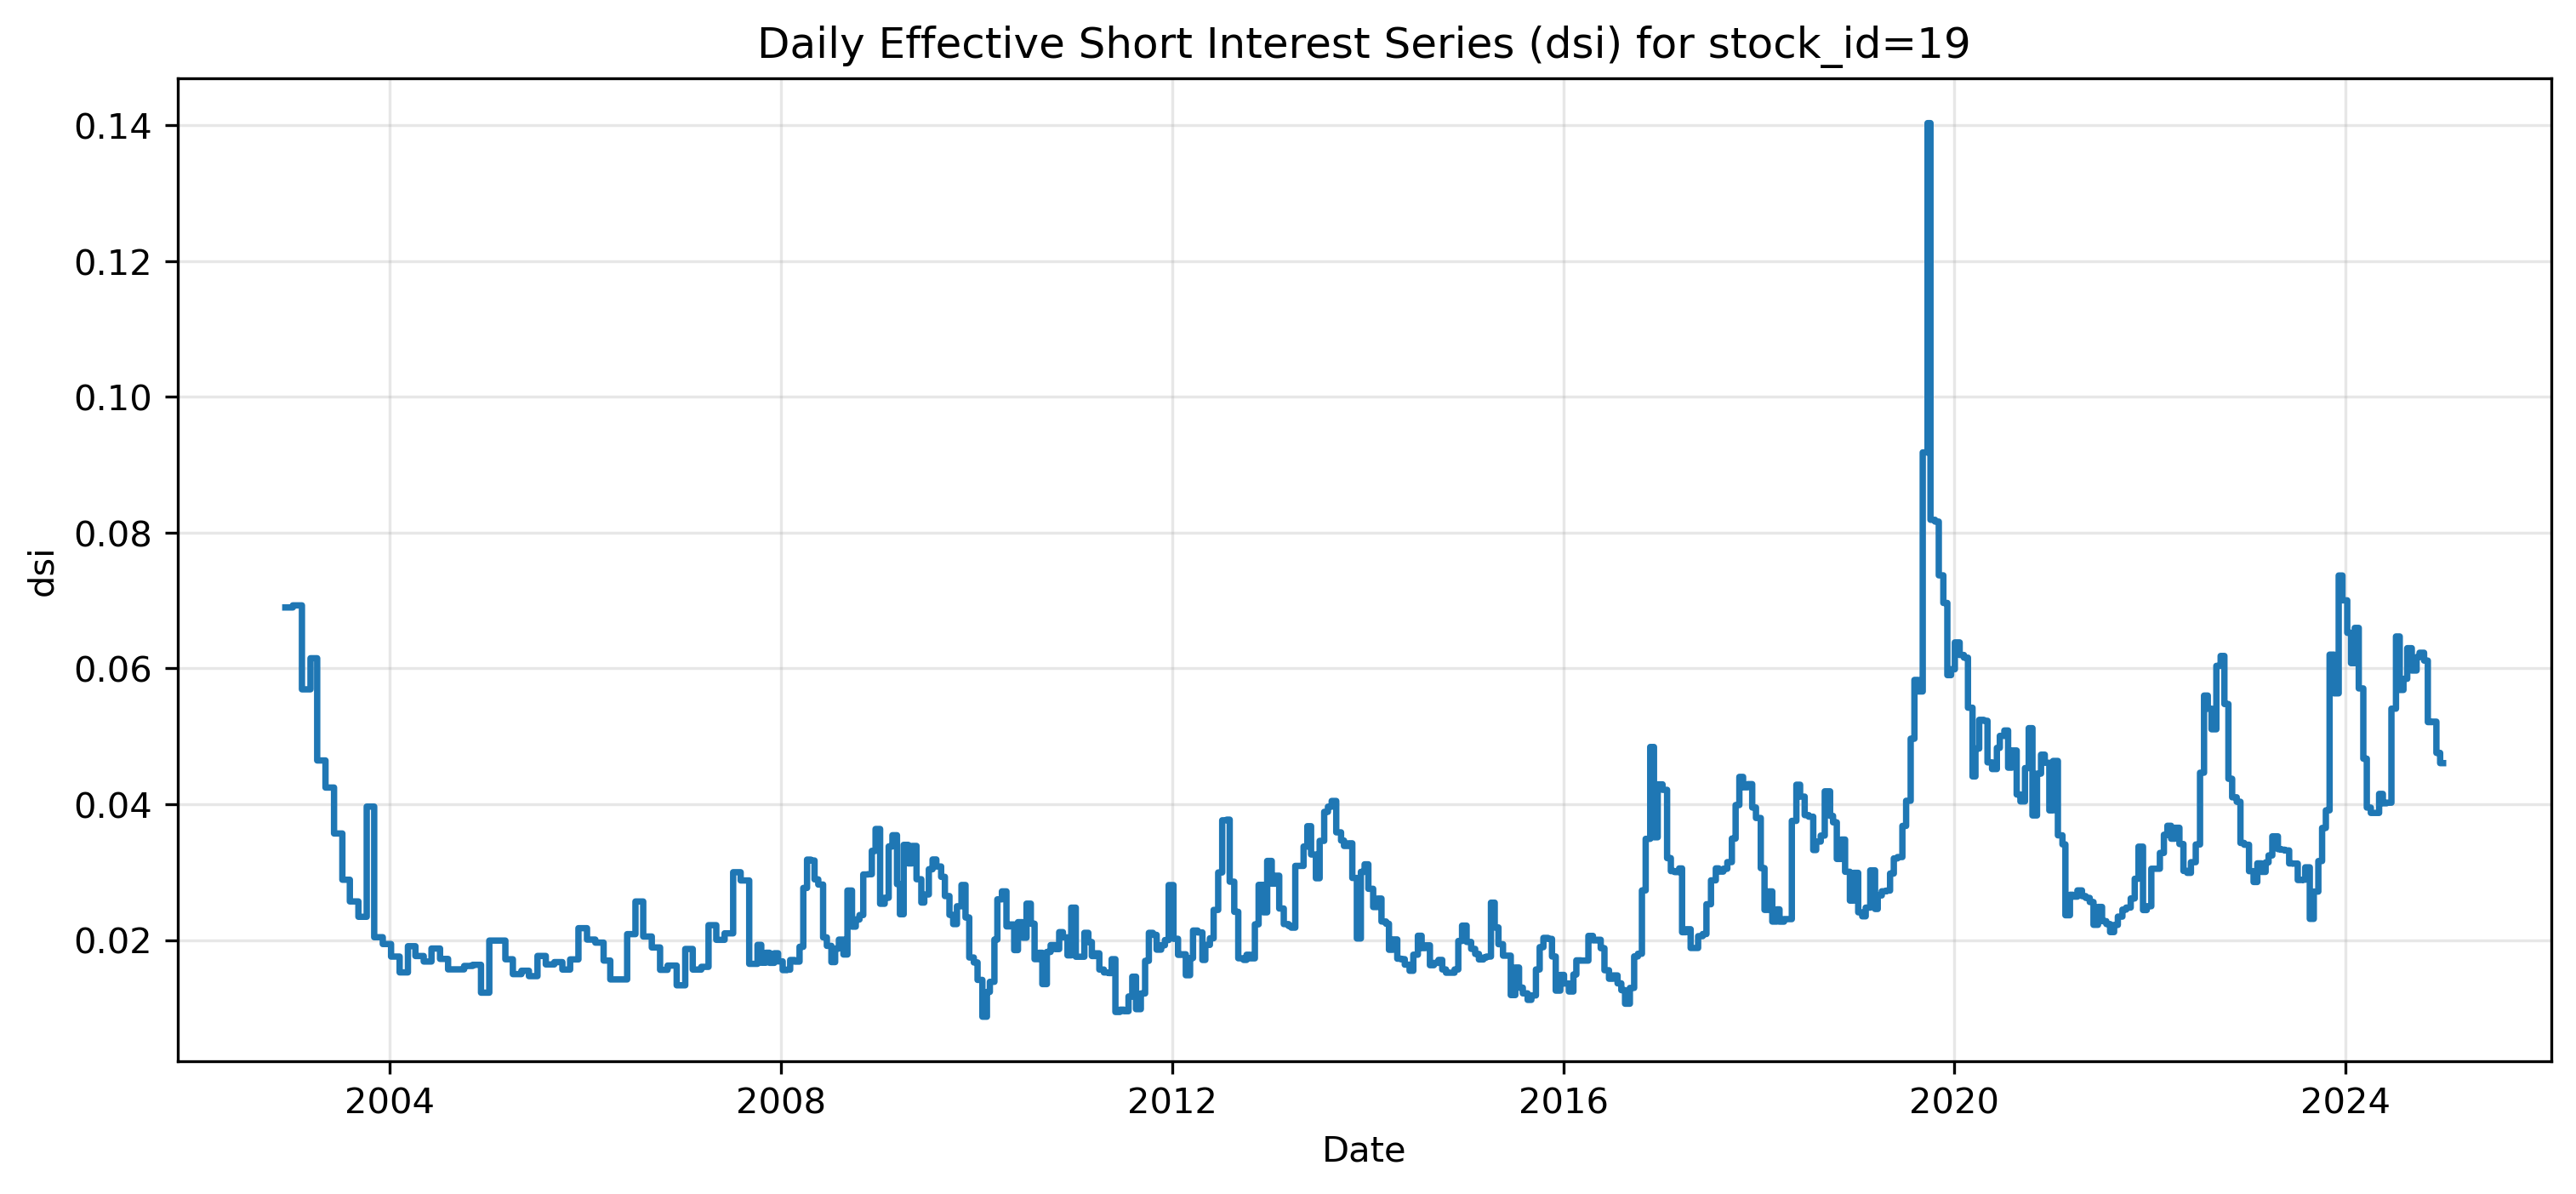
\includegraphics[width=0.9\textwidth]{2.4.png}
\caption{Short interest series for ticker DVA }
\label{fig:pic2.4}
\end{figure}

\subsection{Eligible universe evolve}

The eligible universe expands gradually from 848 names in 2001 to the full 1,000 names by 2007, reflecting the 12-month history requirement and limited coverage in the early sample. From 2007 onward, the annual universe is stable at 1,000 stocks. Mid-year exits are very rare, with only a handful occurring between 2001 and 2007 and none from 2008 to 2024. Overall, this suggests that the point-in-time annual universe construction is stable and only minimally affected by within-year delistings.

 
\begin{table}[H]
\centering
\caption{eligible universe evolve year by year}
\label{tab:2.5}
\begin{tabular}{lrrr}
\toprule
year& eligible\_names& mid\_year\_exits& year\_end\_surviving \\
\midrule
2001& 848& 2& 846
 \\
2002& 869& 2& 867
 \\
2003& 894& 0& 894
 \\
2004& 925& 1& 924
 \\
2005& 947& 0& 947
 \\
2006& 983& 0& 983
\\
2007& 1000& 1&999
\\
2008 - 2024& 1000& 0&1000
\\
\bottomrule
\end{tabular}
\end{table}

\subsection{Portfolio performance }
In the equal-weighted portfolio, all three cumulative return series rise over time. The close-to-close series performs best overall, while both overnight and intraday returns are positive and contribute materially to total performance. Intraday returns are not flat or negative; they grow strongly in the early and middle parts of the sample, with visible drawdowns around 2008–2009 and 2020. Overnight returns rise more gradually at first, then strengthen after 2012 and overtake intraday only late in the sample.

In the value-weighted portfolio, the pattern is closer to the standard stylised fact. The overnight component clearly dominates the long-run growth, while the intraday component remains positive but much smaller. The close-to-close series stays highest throughout, as expected. Overall, the comparison suggests that the overnight premium is much more evident in a large-cap, value-weighted setting than in an equal-weighted stock universe.

\begin{figure}[H]
    \centering
    \begin{minipage}{0.48\textwidth}
        \centering
        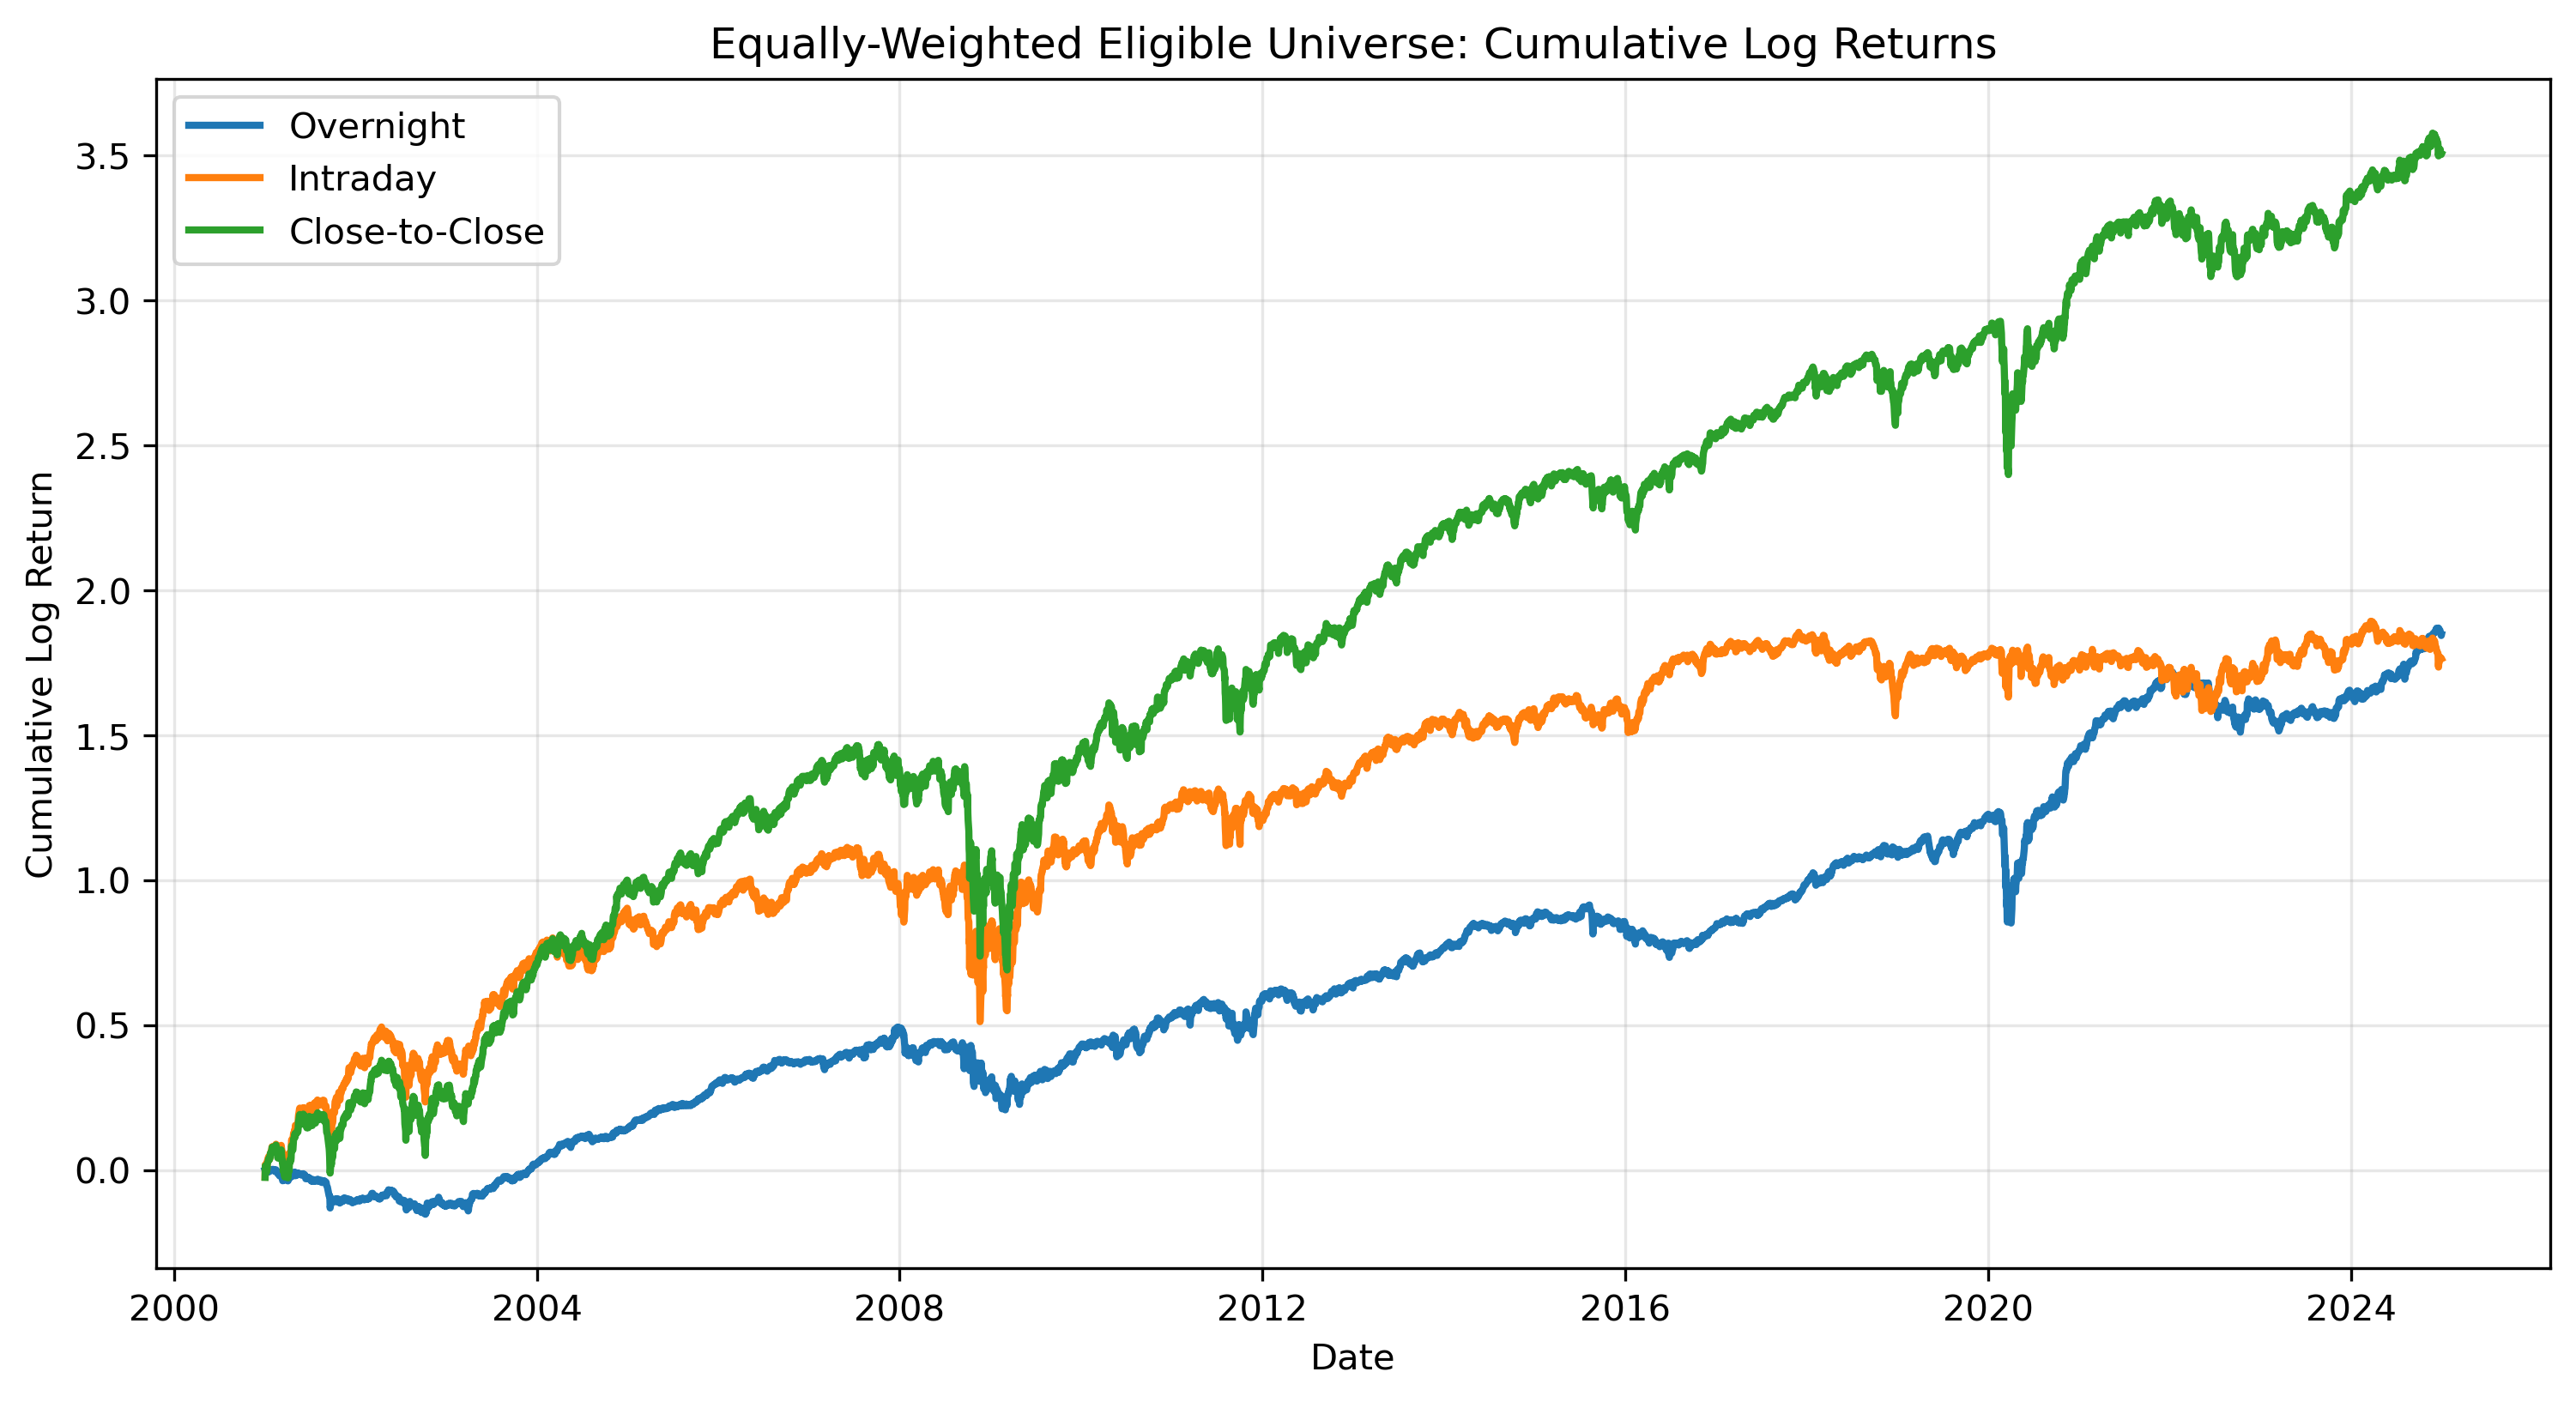
\includegraphics[width=\linewidth]{2.6.1.png}
    \end{minipage}
    \hfill
    \begin{minipage}{0.48\textwidth}
        \centering
        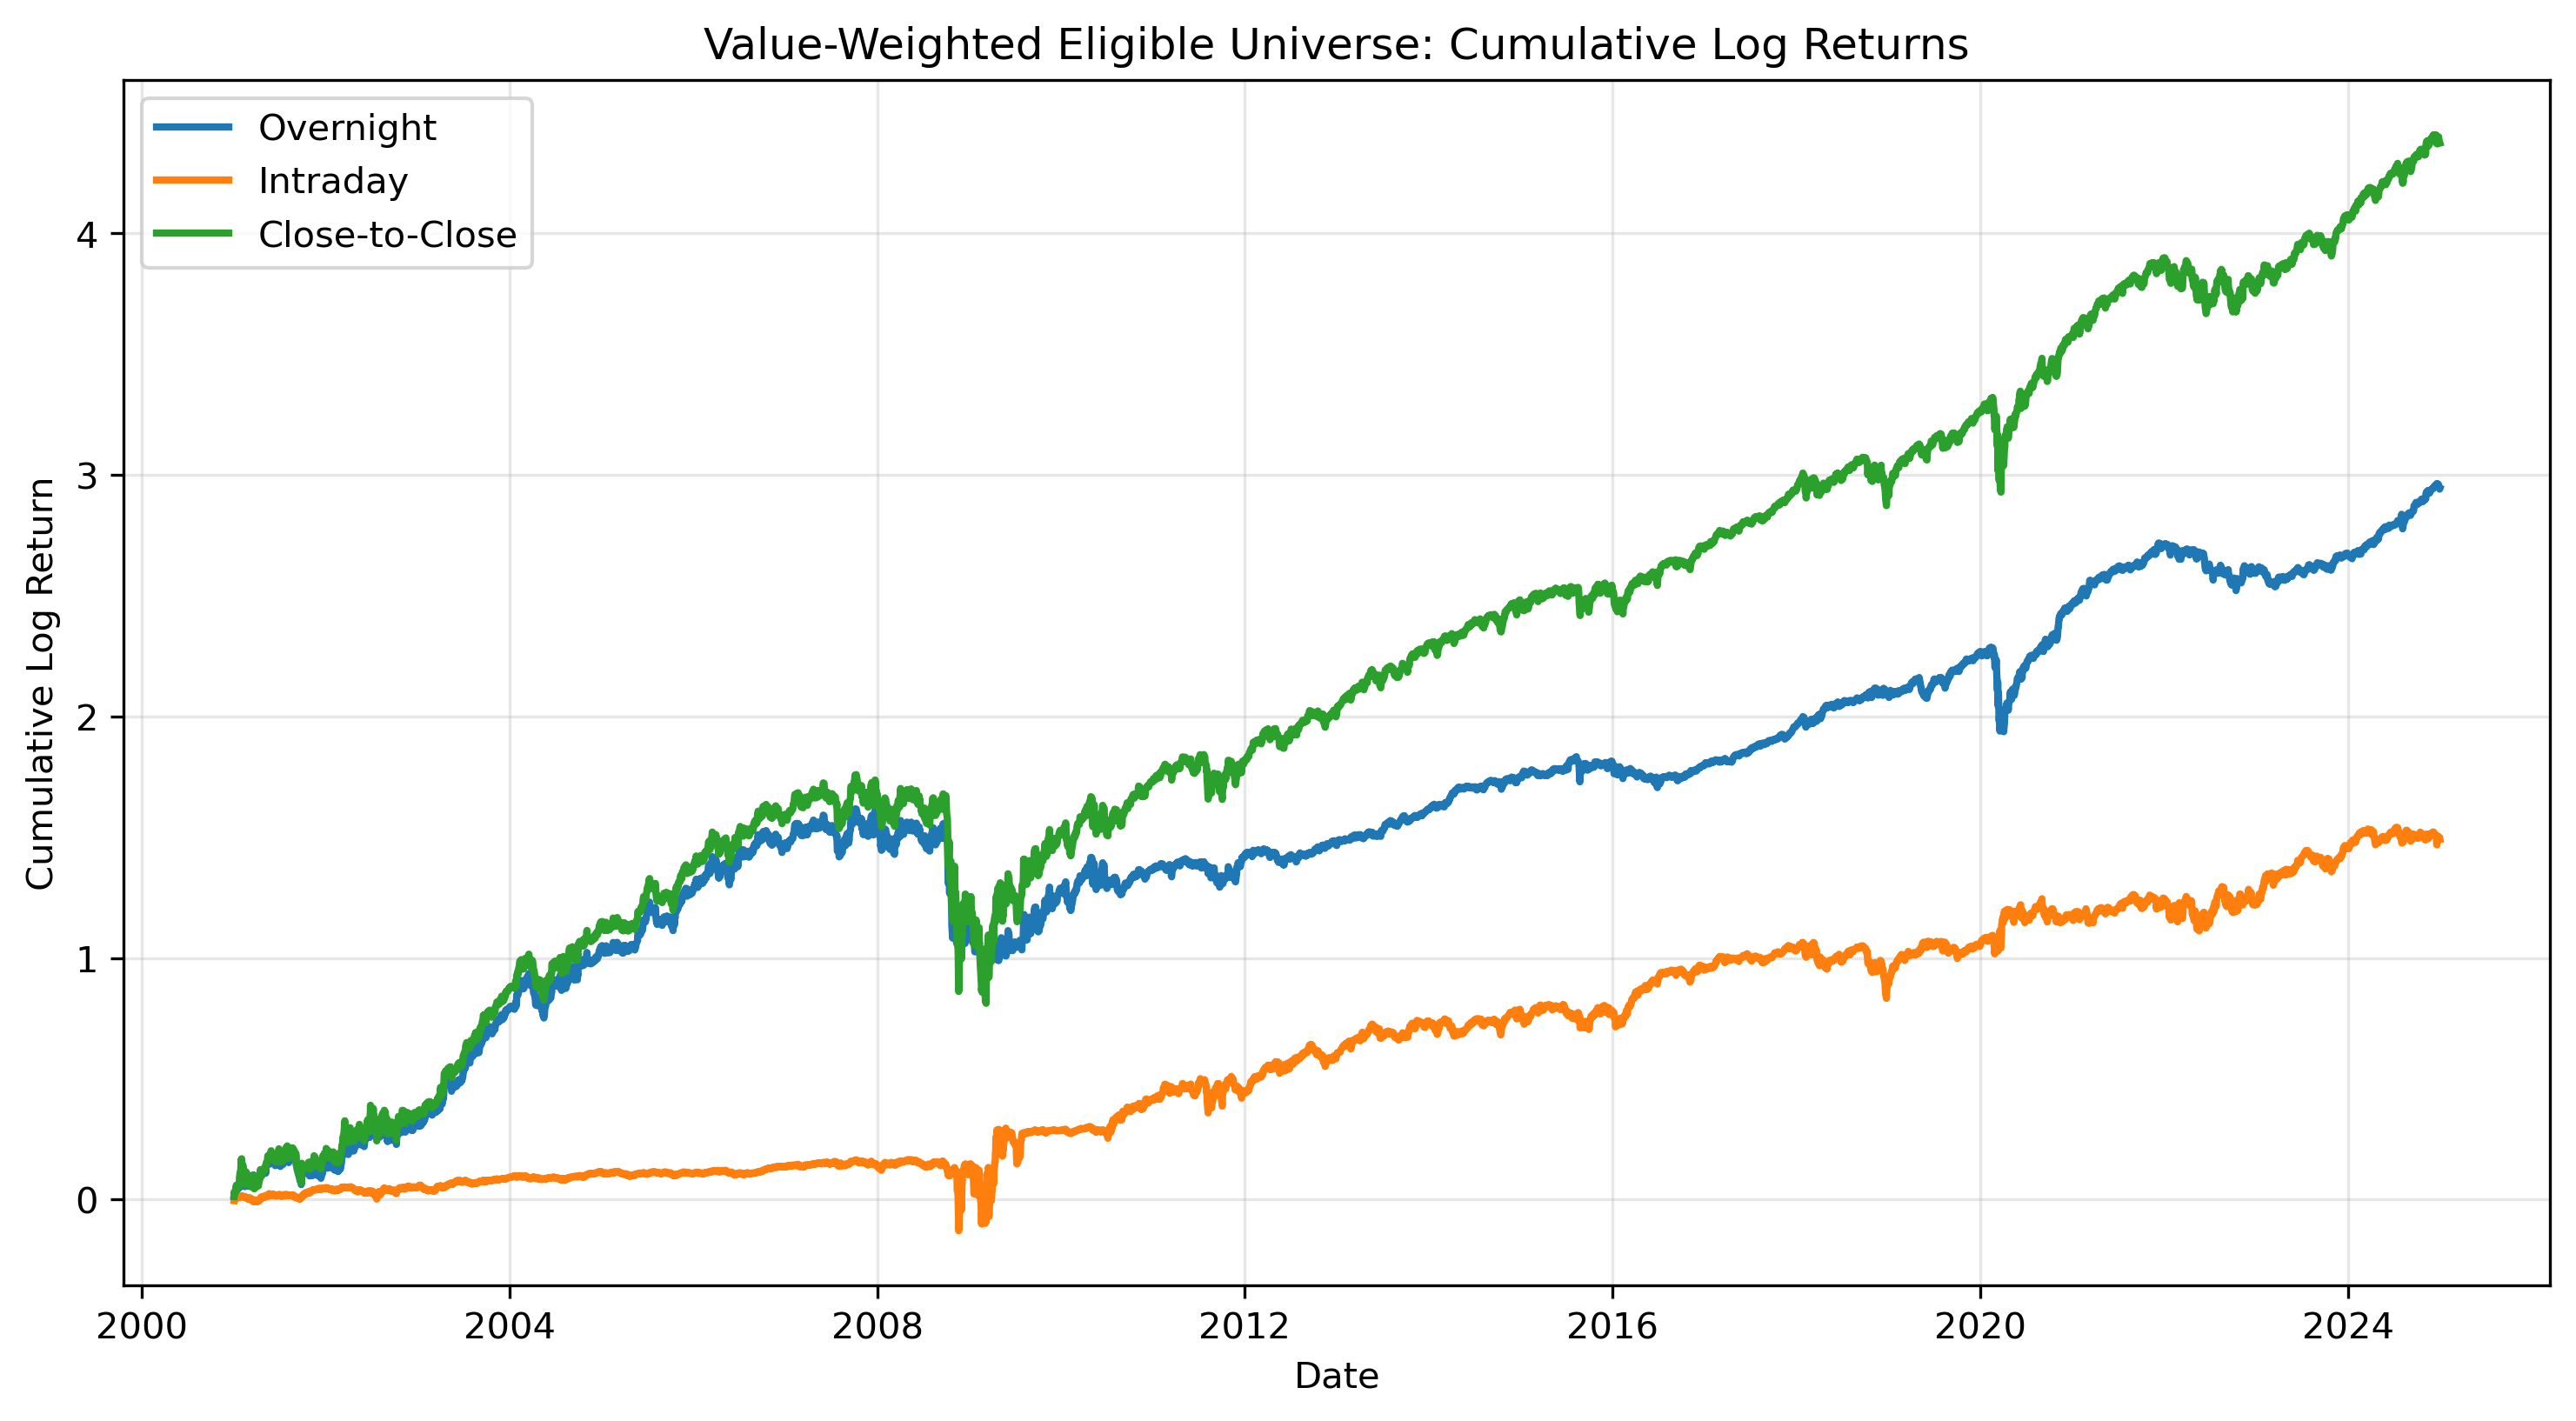
\includegraphics[width=\linewidth]{2.6.2.png}
    \end{minipage}
    \caption{Equally and value weighted portfolio performance}
    \label{fig:2.6 portfolio performance}
\end{figure}

\begin{figure}[H]
    \centering
    \begin{minipage}{0.48\textwidth}
        \centering
        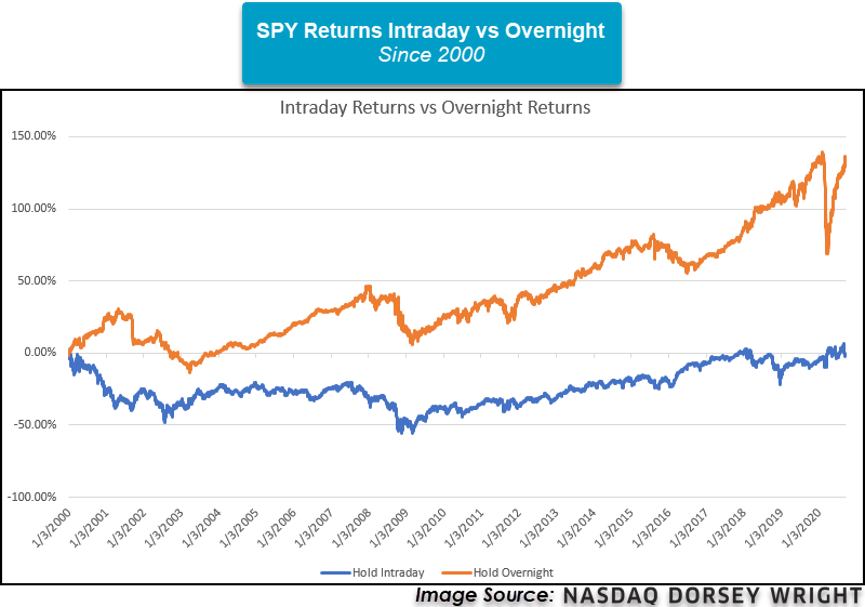
\includegraphics[width=\linewidth]{2.6.3.png}
    \end{minipage}
    \hfill
    \caption{SPF ETF performance, source: \href{https://www.nasdaq.com/articles/overnight-returns-in-a-world-of-volatility-2020-10-08}{Overnight Returns in a World of Volatility | Nasdaq} }
    \label{fig:2.6 SPF ETF performance}
\end{figure}
Our equal-weighted universe does not reproduce the textbook shape exactly: overnight returns are positive, but intraday returns are also positive rather than flat or negative. We do not believe this is mainly a data-cleaning failure. First, the overnight / intraday / close-to-close decomposition reconciles numerically almost perfectly, so the return construction itself is internally consistent. Second, intraday returns are measured from the adjusted open to the adjusted close on the same day, so they are much less exposed than overnight returns to mechanical distortions from splits, dividends, or other corporate actions across trading sessions.

A more plausible explanation is that the stylised fact is fundamentally closer to a large-cap, value-weighted index result than to an equal-weighted stock-level universe result. The lecturer’s figure is presented at the index level, and external evidence based on SPY / S\&P 500 also points to a market-cap-weighted phenomenon. In our results, the value-weighted portfolio is much closer to that benchmark shape than the equal-weighted portfolio, suggesting that the anomaly is strongest among large-cap stocks and is diluted or offset when small and mid-cap names receive equal weight. Therefore, the failure of the equal-weighted universe to match the illustrative chart exactly should not by itself be interpreted as proof that the panel construction is wrong.

 
\begin{table}[H]
\centering
\caption{Dispersion across years}
\label{tab:2.5}
\begin{tabular}{lrrrlll}
\toprule
& on\_ew& id\_ew& c\_to\_c\_ew& on\_vw& id\_vw&c\_to\_c\_vw\\
\midrule
mean& 0.077& 0.073& 0.146
 & 0.123& 0.062&0.182
\\
std& 0.106& 0.145& 0.176
 & 0.162& 0.080&0.185
\\
min& -0.175& -0.196& -0.330
 & -0.417& -0.136&-0.440
\\
max& 0.261& 0.380& 0.455
 & 0.486& 0.223&0.528
\\
2001-2009 mean& 0.047& 0.123&  0.160& 0.142& 0.032&0.169\\
2010-2024 mean& 0.095& 0.044&  0.138
& 0.112& 0.081&0.191
\\
\bottomrule
\end{tabular}
\end{table}


\section{Step 2: Defining a Capacity-Aware Universe }

\subsection{Capacity-aware tradable universe}

Starting from the point-in-time annual universe constructed in Step 1, we further impose daily tradability and capacity filters before any alpha model is trained. The purpose of this step is not to predict returns, but to define the set of stocks that can realistically be traded at the closing auction under the portfolio sizes considered in the brief.

Because the strategy holds positions only overnight and rebuilds the portfolio every trading day, tradability must be defined at the stock-date level rather than as a static list of names. Under the daily-data-only constraint, we do not observe auction-level depth, intraday spreads, or order-book liquidity. We therefore use lagged daily proxies: previous adjusted close, trailing ADV20, lagged realised volatility, year-start market capitalisation, and earnings-calendar flags. These filters are fixed before alpha modelling and are not tuned to maximise in-sample Sharpe; their purpose is to create a conservative and auditable trading universe.

The base universe is the frozen yearly top-1000 universe from Step 1. On each trading day, a stock is allowed to enter the tradable pool only if it passes five filters: a year-start market-capitalisation floor, a lagged price floor, a lagged dollar-volume floor, a realised-volatility band, and an earnings-window exclusion. All filters are constructed using information available before the 15:50 ET decision time. In particular, the price, liquidity and volatility variables are shifted by one trading day, so that full-day close or volume information from day $t$ is not used when forming the portfolio for the close of day $t$.

For each stock $i$ and date $t$, the 20-day average daily dollar volume is defined as
\[
ADV20_{i,t}
=
\frac{1}{20}
\sum_{j=1}^{20}
Close^{adj}_{i,t-j} \times Volume^{adj}_{i,t-j}.
\]
The price filter uses $Close^{adj}_{i,t-1}$, and the realised-volatility filter uses the annualised standard deviation of close-to-close returns over a 60-day rolling window ending at $t-1$:
\[
\sigma^{ann}_{i,t}
=
\sqrt{252}\,
\mathrm{sd}
\left(
r^{CC}_{i,t-60}, \ldots, r^{CC}_{i,t-1}
\right).
\]
We require at least 40 non-missing observations in this 60-day window. This creates a short warm-up period at the beginning of the development sample, which is recorded explicitly as \texttt{MISSING\_LOOKBACK} rather than silently dropped.

The thresholds used in the headline Stage 2 universe are reported in Table~\ref{tab:stage2_thresholds}. They are deliberately simple and conservative. The price and ADV filters remove low-price and low-liquidity names whose auction execution is likely to be unreliable. The market-capitalisation floor is applied at year start, consistent with the frozen-universe construction. The volatility band removes stale or extremely unstable names. The earnings filter removes a one-trading-day window around earnings availability dates, reducing event-risk contamination before the alpha model is trained.

We do not impose a separate Roll-spread filter in the headline universe. Daily Roll-style spread estimates are noisy at the individual-stock level, so we rely on lagged ADV20, price, volatility and the explicit square-root impact model for the hard tradability screen. Spread-style information may still be used later as a modelling feature, but it is not used as a hard exclusion rule in Stage 2.

\begin{table}[htbp]
\centering
\small
\begin{tabular}{lll}
\hline
Filter & Threshold & Point-in-time construction \\
\hline
Price floor & \$5 & Previous adjusted close, $Close^{adj}_{t-1}$ \\
Dollar-volume floor & \$10 million & Lagged $ADV20$ using days $t-20$ to $t-1$ \\
Year-start market cap & \$1 billion & Frozen at previous year-end ranking date \\
Realised volatility & 5\% to 150\% p.a. & Lagged 60-day close-to-close volatility \\
Earnings window & $\pm$ 1 trading day & Around earnings availability date \\
Participation cap & 5\% of $ADV20$ & Applied to each stock-date position limit \\
\hline
\end{tabular}
\caption{Stage 2 eligibility filters and capacity assumptions.}
\label{tab:stage2_thresholds}
\end{table}

Each stock-date receives a single eligibility label. If all filters are passed, the label is \texttt{OK}; otherwise the first binding failure is recorded as \texttt{MCAP\_FAIL}, \texttt{PRICE\_FAIL}, \texttt{ADV\_FAIL}, \texttt{VOL\_FAIL}, \texttt{EARN\_WINDOW}, or \texttt{MISSING\_LOOKBACK}. This creates an auditable eligibility table rather than an opaque filtered sample.

These filters are intended to capture basic tradability rather than to improve the back-test mechanically. The \$5 price floor, \$10 million ADV20 floor and \$1 billion year-start market-cap floor keep the universe focused on reasonably liquid US large-cap stocks. The 5\%--150\% realised-volatility band removes stale or extreme observations, while the $\pm 1$ trading-day earnings window reduces contamination from earnings announcements. The 5\% ADV20 participation cap then turns liquidity into a stock-date-specific capacity constraint instead of assuming that every eligible stock can absorb the same dollar position.

\subsection{AUM scaling and participation cap}

The brief requires the strategy to be reported at three portfolio-AUM levels: \$50 million, \$250 million and \$1 billion. We therefore compute position limits separately for each AUM level. The binary eligibility flag is AUM-invariant: a stock that passes the liquidity, price, volatility, market-cap and earnings filters remains tradable at all three AUM levels. AUM enters through the per-stock position limit and therefore changes the binding-constraint distribution, not the membership of the eligible set.

Assuming a basket of 100 long names and 100 short names, the equal-weight target notional per stock is
\[
q^{target}(AUM) = \frac{AUM}{2 \times 100}.
\]
The per-stock participation constraint is
\[
q^{ADV}_{i,t} = 0.05 \times ADV20_{i,t}.
\]
The maximum allowed position in stock $i$ on date $t$ is then
\[
q_{i,t}(AUM) =
\min\left(
q^{target}(AUM), q^{ADV}_{i,t}
\right).
\]
If $q^{ADV}_{i,t} < q^{target}(AUM)$, the binding constraint is recorded as \texttt{PARTICIPATION\_CAP}; otherwise it is recorded as \texttt{TARGET\_WEIGHT}. This distinction matters because the tradable set may be the same across AUM levels, but the usable position size is not. At higher AUM, more stock-days are constrained by auction capacity.

By construction, the position limit satisfies $q_{i,t} \leq 0.05 \times ADV20_{i,t}$ for every stock-date. Thus no candidate position produced by the Stage 2 sizing rule exceeds the 5\% ADV cap. The final portfolio-construction step later redistributes unused capital subject to the same cap.

\subsection{Universe evolution and exclusion reasons}

Table~\ref{tab:stage2_yearly} summarises the evolution of the capacity-aware universe over selected years. The base universe is approximately 1,000 names throughout the development window. The number of eligible names rises over time as the coverage becomes more liquid and the market-capitalisation floor becomes less restrictive. The lower average in 2010 is mainly due to the rolling-window warm-up period and the \$1 billion year-start market-capitalisation threshold.

\begin{table}[htbp]
\centering
\small
\begin{tabular}{rrrr}
\hline
Year & Avg. base names & Avg. eligible names & Max eligible names \\
\hline
2010 & 1000.0 & 521.0 & 657 \\
2014 & 1000.0 & 833.8 & 886 \\
2018 & 1000.0 & 924.2 & 977 \\
2020 & 1000.0 & 915.9 & 978 \\
2022 & 1000.0 & 941.9 & 992 \\
2024 & 1000.0 & 946.0 & 997 \\
\hline
\end{tabular}
\caption{Evolution of the Stage 2 capacity-aware universe in selected years.}
\label{tab:stage2_yearly}
\end{table}

Across the 2010--2024 development window, the Stage 2 eligibility table contains 3,171,067 \texttt{OK} stock-days. The main exclusion reason is insufficient dollar volume, followed by the year-start market-capitalisation floor and the earnings-window filter. Table~\ref{tab:stage2_reasons} reports the aggregate stock-day counts by exclusion reason.

\begin{table}[htbp]
\centering
\small
\begin{tabular}{lr}
\hline
Eligibility reason & Stock-days \\
\hline
OK & 3,171,067 \\
ADV\_FAIL & 214,507 \\
MCAP\_FAIL & 171,587 \\
EARN\_WINDOW & 117,686 \\
MISSING\_LOOKBACK & 56,720 \\
PRICE\_FAIL & 38,830 \\
VOL\_FAIL & 3,574 \\
\hline
\end{tabular}
\caption{Aggregate Stage 2 eligibility outcomes over 2010--2024.}
\label{tab:stage2_reasons}
\end{table}

For readability, the main text reports aggregate and representative rows. The complete year-by-year exclusion table is reported in Appendix Table~\ref{tab:stage2_reason_by_year}. The AUM-specific binding-constraint distribution is reproducible from \texttt{stage2\_binding\_summary.csv}, and the main text reports the aggregate binding counts by AUM in Table~\ref{tab:stage2_binding}.

\subsection{Capacity impact across AUM levels}

The binding constraint distribution changes materially with AUM. At \$50 million AUM, every eligible stock-day is limited by the equal-weight target rather than the participation cap. At \$250 million, the participation cap binds for 512,517 eligible stock-days. At \$1 billion, the participation cap binds for 1,740,856 eligible stock-days, exceeding the number of target-weight-constrained stock-days. This confirms that capacity is not a cosmetic adjustment: it materially affects the usable position size at institutional AUM levels.

\begin{table}[htbp]
\centering
\small
\begin{tabular}{lrr}
\hline
AUM & TARGET\_WEIGHT stock-days & PARTICIPATION\_CAP stock-days \\
\hline
\$50M & 3,171,067 & 0 \\
\$250M & 2,658,550 & 512,517 \\
\$1B & 1,430,211 & 1,740,856 \\
\hline
\end{tabular}
\caption{Binding position-size constraints by portfolio AUM. Counts are computed over eligible stock-days only.}
\label{tab:stage2_binding}
\end{table}

We also compute the implied auction slippage under the square-root impact convention:
\[
Impact_{i,t}
\approx
k \times \sigma^{daily}_{i,t} \times \sqrt{f} \times 10^4,
\]
where $k=0.7$, $f=5\%$, and $\sigma^{daily}_{i,t}=\sigma^{ann}_{i,t}/\sqrt{252}$. Since auction-level volume is unavailable under the daily-data constraint, we use ADV20 as the capacity proxy and apply the square-root impact convention specified in the brief. Table~\ref{tab:stage2_slippage} reports representative values. The lower-ranked half of the universe has lower ADV and higher volatility, and therefore has higher implied impact than the top-ranked large-cap half.

\begin{table}[htbp]
\centering
\small
\begin{tabular}{llrrr}
\hline
Year & Market-cap bucket & Median impact (bps) & Median ADV20 & Median ann. vol. \\
\hline
2020 & Rank 1--500 & 36.9 & \$202.6M & 37.4\% \\
2020 & Rank 501--1000 & 46.1 & \$36.9M & 46.7\% \\
2024 & Rank 1--500 & 23.9 & \$274.8M & 24.2\% \\
2024 & Rank 501--1000 & 29.8 & \$59.2M & 30.2\% \\
\hline
\end{tabular}
\caption{Representative square-root impact estimates at the 5\% participation cap. The assumptions are daily-data liquidity proxies, 100 names per side, and no use of intraday auction-volume data.}
\label{tab:stage2_slippage}
\end{table}

Overall, Stage 2 converts the annual top-1000 universe into a daily tradable universe with explicit capacity limits. The resulting table is used by the later modelling and portfolio-construction stages: alpha scores are generated only for \texttt{is\_trade\_eligible == True} names, while position sizing uses the AUM-specific position limits computed here. This ensures that the subsequent back-test does not implicitly assume infinite liquidity or ignore auction-capacity constraints.



\section{Step 3: Filtering the Short Leg for Borrow Cost}

Long positions can buy any large-cap stock at the closing auction without restriction. Short positions cannot. A short sale requires borrowing shares, and the lender charges a borrow fee. For most large-cap stocks this fee matches the General Collateral (GC) rate of roughly 25 to 50 basis points per year. For some stocks the fee reaches several hundred basis points. This scenario typically occurs when short-selling interest is high, liquidity is scarce, and short-selling pressure increases risks. If the short book concentrates in such stocks, the borrow cost can fully offset the alpha. We therefore build a hard-to-borrow (HTB) proxy that is free of look-ahead bias. We base it on the Step 2 tradable pool and the Step 1 point-in-time short-interest data. We then map it onto the prescribed three-tier borrow-cost schedule. Every input we use is observable by 15:50~ET, so the proxy uses no future information.



\subsection{The Hard-to-Borrow Proxy}
\label{sec:step3q1}

We construct our point-in-time hard-to-borrow (HTB) proxy from three short-interest variables in the daily short-interest dataset.

\begin{itemize}
  \item \texttt{dsi} (short interest / shares outstanding) captures the imbalance
        between short demand and lendable supply.
  \item \texttt{dtcn} (days-to-cover) measures how crowded the short positions are
        relative to market liquidity.
  \item \texttt{ddtcn} (change in days-to-cover) captures acute deterioration in
        lending conditions and acts as a stress signal.
\end{itemize}

We calibrate the thresholds from the cross-sectional distribution of the Step~2
eligible universe. \texttt{dsi} reaches about $0.09$ at the 90th percentile and
about $0.20$ at the 99th. \texttt{dtcn} reaches about $9.5$ at the 90th percentile
and about $21.5$ at the 99th. We then define the following absolute economic gates.

\begin{itemize}
  \item \textbf{Hard-to-borrow (Tier~B floor):} \texttt{dsi}~$\geq 0.10$ \emph{or}
        \texttt{dtcn}~$\geq 10$. The 10\%-of-float level is the borrow-risk marker
        that the brief itself references. Ten days-to-cover corresponds to roughly
        two trading weeks.
  \item \textbf{Deep special (Tier~C):} \texttt{dsi}~$\geq 0.20$ \emph{or}
        \texttt{dtcn}~$\geq 20$; \emph{or} a near-deep name
        (\texttt{dsi}~$\geq 0.15$ or \texttt{dtcn}~$\geq 15$) that also sits in the
        top decile of the daily cross-section of rising \texttt{ddtcn} (positive
        change in days-to-cover).
\end{itemize}

We combine the variables deliberately. We use \emph{or} between \texttt{dsi} and
\texttt{dtcn} because each measures a distinct dimension of borrow scarcity, and
either tail alone makes a name expensive to borrow. We bind the \texttt{ddtcn}
stress term to a near-deep condition with \emph{and}, because \texttt{ddtcn} is a
noisy change variable. This ensures that stress can only elevate a name into Tier C when its level variables are already close to the deep-special range, rather than letting the stress term act on its own. We
compute the stress term within each daily cross-section, so the rule stays point-in-time. Tier~C remains a small subset of the eligible pool (about $3.45\%$ of stock-days).

We use absolute economic thresholds rather than relative ranks on purpose. These
fixed values reproduce on the held-out 2025--2026 window without any recalibration, so the rule introduces no look-ahead and the proxy stays consistent across the development and held-out samples.


\subsection{External Validation}

A meaningful proxy should surface documented hard-to-borrow or crowded-short names without hard-coding any ticker. We rank names by their number of Tier~C
days in Table~\ref{tab:step3-top-tierc}. GME is the clearest case. It was the centre of the widely studied January~2021 short squeeze, driven by exceptionally
high short interest in a heavily crowded short \cite{malz2021gamestop}. Our proxy flags GME
as crowded-short well before 2021. This timing suggests that the rule captures
pre-existing short-supply pressure. It does not simply react to the event ex post. This is supportive rather than definitive validation, because we do not observe actual stock-loan fees.
\begin{table}[H]
\centering
\caption{Top names by number of Tier-C trading days under the Step~3
hard-to-borrow proxy. Sample: trade-eligible stock-days, 2010--2024.}
\label{tab:step3-top-tierc}
\begin{tabular}{lrrrrll}
\toprule
Ticker & Tier-C days & Mean dsi & Max dsi & Mean dtcn & First date & Last date \\
\midrule
FFIN & 2500 & 0.1124 & 0.1787 & 37.87 & 2010-03-03 & 2024-11-20 \\
ENOV & 1557 & 0.2832 & 0.5524 & 33.04 & 2012-01-11 & 2022-02-04 \\
GME  & 1276 & 0.2861 & 0.4792 & 15.12 & 2013-04-02 & 2024-05-03 \\
GATX & 1186 & 0.1996 & 0.3302 & 28.16 & 2010-03-11 & 2020-12-31 \\
PRAA & 1110 & 0.1905 & 0.2811 & 27.65 & 2011-01-03 & 2017-12-29 \\
\bottomrule
\end{tabular}
\end{table}

\subsection{Tier-to-Cost Mapping}
We map each tier onto the borrow-cost schedule specified in the brief's Section~6.3 (Table~\ref{tab:step3-tiers}). We charge the daily equivalent (annual rate $\div\,252$) on the gross short notional of each name held short
overnight in Step~5.


\begin{table}[ht]
  \centering
  \begin{tabular}{llr}
    \toprule
    Tier & Meaning & Rate (bps p.a.) \\
    \midrule
    A & General Collateral (not HTB)               & 40  \\
    B & Mid-tier special (moderate-confidence HTB)  & 200 \\
    C & Deep special (high-confidence HTB)          & 800 \\
    \bottomrule
  \end{tabular}
  \caption{Borrow-tier cost schedule, fixed by the brief in its Section~6.3. We charge the daily equivalent (annual rate $\div\,252$) on the gross
  short notional of each name held overnight, and we assign tiers from the
  Step~3 HTB proxy of Section~\ref{sec:step3q1}.}
  \label{tab:step3-tiers}
\end{table}

\subsection{Tiered cost vs. Hard Exclusion}

We adopt a tiered cost treatment rather than a hard exclusion rule. A hard exclusion is conservative. It may also discard genuine alpha when the proxy misclassifies a stock. Tiered costing is more flexible. High-cost names can still enter the short book. Their realised returns then fall by the corresponding borrow fee in Step~5.

About 13\% of eligible stock-days over the full sample are classified as hard-to-borrow (Tier~B or Tier~C), and about 3.5\% are classified as deep specials (Tier~C). Table~\ref{tab:stage3-tier-yearly} reports the annual breakdown. These shares describe the tradable universe before portfolio construction.

The fraction directly requested in Q3 is measured after the raw short signal is formed. The raw short signal is the bottom tail of the Step~4 cross-sectional alpha score, selected as the short basket in Step~5. A short candidate is affected by the borrow treatment if its assigned tier is B or C. We calculate this fraction in Step~5, after the final alpha score and basket width are fixed. The specific method involves merging the Step~3 borrow-tier table into the raw short basket.

\begin{table}[H]
\centering
\caption{Annual borrow-tier shares of the trade-eligible universe. Shares are
computed over eligible stock-days before final short-book construction.}
\label{tab:stage3-tier-yearly}
\begin{tabular}{rrrrr}
\toprule
Year & Tier A (\%) & Tier B (\%) & Tier C (\%) & HTB share (\%) \\
\midrule
2010 & 82.64 & 12.58 & 4.79 & 17.36 \\
2011 & 83.88 & 11.80 & 4.32 & 16.12 \\
2012 & 84.80 & 10.81 & 4.39 & 15.20 \\
2013 & 83.26 & 10.35 & 6.40 & 16.74 \\
2014 & 82.75 & 11.48 & 5.77 & 17.25 \\
2015 & 83.34 & 11.74 & 4.92 & 16.66 \\
2016 & 81.61 & 13.35 & 5.04 & 18.39 \\
2017 & 81.81 & 13.26 & 4.92 & 18.19 \\
2018 & 85.12 & 11.53 & 3.35 & 14.88 \\
2019 & 85.98 & 10.56 & 3.47 & 14.02 \\
2020 & 89.68 & 7.84 & 2.49 & 10.32 \\
2021 & 92.52 & 6.02 & 1.46 & 7.48 \\
2022 & 94.49 & 4.52 & 0.98 & 5.51 \\
2023 & 93.60 & 5.52 & 0.88 & 6.40 \\
2024 & 94.06 & 5.04 & 0.90 & 5.94 \\
\bottomrule
\end{tabular}
\end{table}



\subsection{Gross- versus Net-of-Borrow Sharpe}

The gross- and net-of-borrow Sharpe ratios require realised portfolio returns. Borrow fees apply only to names actually held short. We supplies the
point-in-time borrow tiers and the fixed cost schedule in
Table~\ref{tab:step3-tiers}. Step~5 applies these costs to the realised short book.

We isolate the borrow component directly. The gross-of-borrow Sharpe charges commission and auction slippage but no borrow fee. It therefore differs from the
cost-free Gross SR column in Table~\ref{tab:step5-headline}. The net-of-borrow Sharpe adds the daily Tier A/B/C borrow charge on short notional. On the
2019--2024 out-of-sample window at 250M AUM, the gross-of-borrow Sharpe is 0.50 and the net-of-borrow Sharpe is 0.47. Borrow therefore reduces the Sharpe by about 0.03 points. The borrow drag is 0.04, 0.03, and 0.02 Sharpe points at 50M, 250M, and 1B respectively. The drag falls as AUM rises. The participation cap reduces
realised exposure to capacity-constrained short names. We report the full comparison across windows and AUM levels in Step~5, Table~\ref{tab:step5-headline}.


\section{Step 4: Constructing the Cross-Sectional Alpha}
\subsection{Information Set, Target, and Feature Construction}

At the decision time of 15:50 ET on day $t$, the model produces a real-valued score $s_{i,t}$ for each stock $i$ in the eligible universe $\mathcal{U}_t$. The purpose of this score is to rank stocks by their expected next-session overnight return. The prediction target is defined as:
\begin{equation}
    y_{i,t} = r_{ON,i,t+1} = \frac{Open^{adj}_{i,t+1}}{Close^{adj}_{i,t}} - 1 .
\end{equation}

This target represents the return from the close of day $t$ to the open of day $t+1$. Since $Open^{adj}_{i,t+1}$ is not observable at 15:50 ET on day $t$, the target is used only for model training and evaluation. It is never included as an input feature.

The information set $\mathcal{F}_t$ contains only information observable at or before 15:50 ET on day $t$. This includes current-day open prices, previous trading-day close prices, lagged returns, lagged volatility and liquidity measures, public short-interest information after applying reporting or publication lags, deterministic calendar information, and cross-sectional ranks computed from point-in-time observable base features. It excludes any information that would only become available after 15:50 ET, such as the final closing price of day $t$, full-day trading volume on day $t$, or the next-day opening price.

The final model uses 75 point-in-time features. These features are grouped into six categories: return-based features, volatility features, liquidity and size features, short-interest features, calendar features, and cross-sectional rank features. The complete line-by-line feature list, formulas, economic meanings, and observability checks are reported in Appendix Table~\ref{tab:feature_appendix}.

Return-based features capture short-term price dynamics, including overnight momentum, close-to-close momentum, intraday effects, and short-term reversal. For example, current-day overnight return is computed using the current-day adjusted open price and the previous-day adjusted close price:
\begin{equation}
    r_{ON,i,t} = \frac{Open^{adj}_{i,t}}{Close^{adj}_{i,t-1}} - 1 .
\end{equation}

This variable is observable at 15:50 ET on day $t$, because both $Open^{adj}_{i,t}$ and $Close^{adj}_{i,t-1}$ are already known. By contrast, any feature requiring the final close of day $t$ is lagged. Therefore, intraday return and close-to-close return features are constructed using $t-1$ or earlier observations when necessary. Rolling return features, momentum features, and reversal features are also computed using only historical observations available by the decision time.

Volatility features measure recent historical risk. They are constructed as rolling standard deviations of past returns, such as 20-day or 60-day historical volatility. These variables are economically motivated because stocks with higher recent volatility may have larger overnight price movements and different risk premia. To avoid look-ahead bias, volatility measures are lagged and use only returns observed before the decision time.

Liquidity and size features capture trading capacity, transaction costs, and firm size. For example, average daily dollar volume is computed using a historical rolling window:
\begin{equation}
    ADV20_{i,t} = \frac{1}{20} \sum_{j=1}^{20} DollarVolume_{i,t-j}.
\end{equation}

The log-transformed liquidity feature is then defined as:
\begin{equation}
    log\_adv20_{i,t} = \log(1 + ADV20_{i,t}).
\end{equation}

This construction avoids using full-day volume on day $t$, which would not be known at 15:50 ET. Size variables, such as market capitalization, are based on point-in-time or year-start information and therefore do not use future prices.

Short-interest features measure short-selling pressure, bearish positioning, and potential short-covering pressure. These include days-to-cover measures, changes in short-interest indicators, and their lagged values. Since short-interest data are not always public immediately on the report date, the raw short-interest information is only used after applying the relevant reporting or publication lag. After this adjustment, the daily panel is forward-filled using only information that would have been public by day $t$. Therefore, these variables are point-in-time and do not use future short-interest information.

Calendar features capture deterministic seasonal effects, such as day-of-week, month, month-start, month-end, and year-end effects. These variables are known in advance from the trading calendar and therefore are observable at 15:50 ET on day $t$. They are included to allow the model to capture systematic patterns related to institutional trading, portfolio rebalancing, and seasonal market effects.

Cross-sectional rank features transform raw signals into daily percentile ranks within the eligible universe. For a base feature $X_{i,t}$, the corresponding rank feature can be written as:
\begin{equation}
    Rank(X_{i,t}) = \frac{rank_t(X_{i,t}) - 1}{N_t - 1},
\end{equation}
where $N_t$ is the number of eligible stocks on day $t$.

These rank features capture the relative position of each stock compared with other tradable stocks on the same day. This is appropriate for a cross-sectional prediction problem because the portfolio construction step depends mainly on the ranking of stocks rather than the absolute level of predicted returns. Cross-sectional ranking does not introduce look-ahead bias as long as the underlying base feature $X_{i,t}$ is observable at 15:50 ET on day $t$.

Overall, the feature set is constructed in a point-in-time manner. The target variable is excluded from the input feature matrix. Current-day overnight features use only prices known by the decision time. Intraday and close-to-close return variables are lagged when necessary. Rolling volatility, liquidity, and momentum variables are computed from historical windows only. Short-interest variables are adjusted for publication lags before being used. Calendar variables are deterministic, and cross-sectional ranks are computed only from observable base features. Therefore, the final 75 features are observable at 15:50 ET on day $t$ and do not introduce look-ahead bias. The detailed feature-level verification is provided in Appendix Table~\ref{tab:feature_appendix}.
\subsection{Model Class and Training Scheme}

We formulate the task as a supervised daily cross-sectional prediction problem. On each trading day $t$, for each stock $i$ in the eligible universe $\mathcal{U}_t$, the model observes a point-in-time feature vector $X_{i,t}\in\mathcal{F}_t$ and outputs a real-valued score
\[
s_{i,t}=f_{\theta}(X_{i,t}),
\]
where a higher score indicates a higher expected next-session overnight return. The target return is
\[
r^{ON}_{i,t+1}=\frac{Open_{i,t+1}}{Close_{i,t}}-1.
\]
In the implementation, the winsorised version of the next overnight return, \texttt{target\_r\_on\_next\_winsor}, is used to reduce the influence of extreme outliers.

After applying the tradability filter \texttt{is\_trade\_eligible == True} and removing observations with missing target values, the final modelling sample contains 3,170,073 stock-date observations and 75 Boruta-selected point-in-time features. The sample is split chronologically, rather than randomly, into training, validation, and test periods.

\begin{table}[H]
\centering
\caption{Chronological sample split}
\begin{tabular}{lll}
\toprule
Split & Date range & Number of observations \\
\midrule
Training & 2010-03-03 to 2018-12-31 & 1,758,771 \\
Validation & 2019-01-02 to 2021-12-31 & 702,218 \\
Test & 2022-01-03 to 2024-12-30 & 709,084 \\
\bottomrule
\end{tabular}
\end{table}

This chronological split is important because the problem is a real-time investment problem. At decision time on day $t$, future data are not available. Therefore, random train-test splitting would create look-ahead bias and would overstate the model's true out-of-sample performance.

\subsubsection{Ridge Regression Benchmark}

The first model is Ridge Regression, which is used as a transparent linear benchmark. The model takes the 75 selected features and predicts the winsorised next overnight return directly:
\[
\hat{r}^{ON}_{i,t+1}
=
\beta_0 + X_{i,t}^{\top}\beta.
\]

The Ridge estimator is obtained by minimising
\[
\sum_{(i,t)\in Train}
\left(
y_{i,t} - \beta_0 - X_{i,t}^{\top}\beta
\right)^2
+
\alpha \sum_{j=1}^{p}\beta_j^2,
\]
where $y_{i,t}=\texttt{target\_r\_on\_next\_winsor}$, $p=75$, and $\alpha$ controls the strength of $L_2$ regularisation.

The Ridge pipeline applies median imputation to missing feature values, standardises all features using \texttt{StandardScaler}, and then fits a Ridge model with an intercept. Standardisation is required because Ridge penalises coefficient magnitudes, so the penalty would not be comparable across features measured on different scales without scaling.

The regularisation parameter $\alpha$ is selected on the validation set. The candidate grid is
\[
\alpha \in 
\{0.001, 0.01, 0.1, 1, 10, 100, 1000, 10000\}.
\]
Because the final objective of the coursework is to rank stocks in the cross-section, the model is selected by validation mean daily Rank IC rather than by RMSE alone. The best value selected by the code is
\[
\alpha = 10000.
\]

After selecting $\alpha$, the Ridge model is first trained on the training period only and evaluated on the validation period. For the final test evaluation, the model is refitted on the combined training and validation periods and then evaluated on the test period. The Ridge prediction \texttt{ridge\_pred\_return} is used directly as the stock score \texttt{ridge\_score}. Stocks with higher \texttt{ridge\_score} are ranked higher and are candidates for the long side of the portfolio, while stocks with lower scores are candidates for the short side.

\subsubsection{XGBoost2 Main Model}

The second model is an XGBoost regression model, which is used as the main nonlinear model. XGBoost is a gradient-boosted decision tree model. Compared with Ridge Regression, it can capture nonlinear effects, threshold effects, and interactions between features without requiring these interactions to be specified manually.

The XGBoost2 model is implemented using \texttt{XGBRegressor} with squared-error loss:
\[
\texttt{objective}=\texttt{reg:squarederror}.
\]

However, unlike Ridge Regression, XGBoost2 is not trained to predict the raw overnight return directly. Instead, the code transforms the winsorised overnight return into a daily cross-sectional rank target:
\[
\texttt{target\_cs\_rank}_{i,t}
=
\operatorname{rank}_{j\in\mathcal{U}_t}
\left(
\texttt{target\_r\_on\_next\_winsor}_{j,t}
\right)
-0.5.
\]
This means that the XGBoost model is trained to predict whether a stock will rank high or low within the same trading day, rather than to predict the exact numerical level of the overnight return. This is more consistent with the portfolio construction problem, because the trading strategy depends primarily on the cross-sectional ordering of stocks.

The XGBoost2 code tests 23 candidate hyperparameter combinations. These combinations vary the number of trees, tree depth, learning rate, subsampling rate, column subsampling rate, minimum child weight, $L_1$ and $L_2$ regularisation, and the \texttt{gamma} split penalty. During tuning, the code uses up to 600,000 randomly sampled training observations to reduce computational cost, while keeping the full validation set for model selection. The random sampling is done only inside the training period, so it does not create look-ahead bias.

The model is selected using validation mean daily Spearman IC as the primary criterion, with validation long-short Sharpe and ICIR used as secondary criteria. This selection rule is appropriate because the purpose of the model is not just to minimise squared error, but to produce a stable and useful daily cross-sectional ranking.

The selected XGBoost2 model is candidate model 20, with the following hyperparameters:

\begin{table}[H]
\centering
\caption{Selected XGBoost2 hyperparameters}
\begin{tabular}{lr}
\toprule
Hyperparameter & Value \\
\midrule
\texttt{n\_estimators} & 400 \\
\texttt{max\_depth} & 5 \\
\texttt{learning\_rate} & 0.02 \\
\texttt{subsample} & 0.80 \\
\texttt{colsample\_bytree} & 0.80 \\
\texttt{min\_child\_weight} & 10 \\
\texttt{reg\_lambda} & 10 \\
\texttt{reg\_alpha} & 0.1 \\
\texttt{gamma} & 0.1 \\
\bottomrule
\end{tabular}
\end{table}

The selected model achieves a validation mean daily Spearman IC of approximately 0.0322 during the tuning stage. In the final run, the model is refitted on the training period only, keeping the validation period as a pure model-selection sample. It then generates predictions for the training, validation, and test periods.

The raw XGBoost prediction is stored as \texttt{pred\_xgboost2}. The code then converts this raw prediction into a daily cross-sectional percentile rank:
\[
\texttt{score\_xgboost2\_rank}_{i,t}
=
\operatorname{rank}_{j\in\mathcal{U}_t}
\left(
\texttt{pred\_xgboost2}_{j,t}
\right).
\]
This final score lies approximately between 0 and 1. A value close to 1 means that the stock is among the most attractive stocks on that day according to the model, while a value close to 0 means that the stock is among the least attractive stocks. This ranked score is the most suitable output for the portfolio construction stage.

\subsubsection{Justification Relative to the Problem Constraints}

The modelling and training scheme is designed to match the three main constraints of the coursework: cross-sectional, daily, and point-in-time.

First, the task is cross-sectional. On each date, the model is required to rank stocks within that day's eligible universe, rather than to forecast a single time series. Therefore, the main evaluation and tuning criteria are daily Rank IC, daily Spearman IC, and long-short portfolio performance. This is why Ridge is selected using validation mean daily Rank IC and XGBoost2 is selected using validation mean daily Spearman IC.

Second, the task is daily. Each observation is a stock-date pair $(i,t)$, and the model produces one score per stock per trading day. The backtest and IC calculations are also computed at the daily level. This matches the actual trading setup, where the signal is formed before the close of day $t$ and used to trade from the close of day $t$ to the open of day $t+1$.

Third, the task is point-in-time. All features used by the models come from the final 75-feature panel, which was constructed to include only information observable at or before 15:50 ET on day $t$. Lagged return variables, volatility measures, liquidity variables, short-interest variables, earnings-calendar features, and calendar features are all aligned so that future information is not used. The model code also explicitly excludes non-feature columns such as \texttt{date}, \texttt{ticker}, \texttt{instrument\_id}, \texttt{sample\_split}, \texttt{is\_trade\_eligible}, \texttt{target\_r\_on\_next}, and \texttt{target\_r\_on\_next\_winsor} from the feature set.

Overall, Ridge Regression provides a simple and interpretable linear benchmark, while XGBoost2 provides a more flexible nonlinear model that is better suited to capturing complex relationships in the 75-feature cross-section. The chronological training-validation-test split, validation-based hyperparameter selection, and daily rank-based evaluation together ensure that the modelling framework is consistent with the real-time, point-in-time nature of the prediction problem.
\subsection{Cross-sectional Information Coefficient}

To evaluate the quality of the model scores, we compute the daily cross-sectional Information Coefficient (IC). Since the task is primarily a ranking problem, we focus on the Spearman rank IC rather than the Pearson correlation. For each test date \(t\), the IC is defined as the cross-sectional rank correlation between the model score \(s_{i,t}\) and the realised next-day overnight return \(r^{ON}_{i,t+1}\) across all eligible stocks:
\[
IC_t =
\operatorname{Corr}^{\text{Spearman}}_i
\left(
s_{i,t}, r^{ON}_{i,t+1}
\right),
\quad i \in \mathcal{U}_t ,
\]
where \(\mathcal{U}_t\) is the eligible trading universe on date \(t\). A positive IC means that stocks assigned higher scores by the model tend to realise higher next-day overnight returns.

The reported t-statistic is computed from the time series of daily ICs:
\[
t(\overline{IC})
=
\frac{\overline{IC}}
{sd(IC_t)/\sqrt{T}},
\]
where \(T\) is the number of test-period trading days. The out-of-sample test period is 2022--2024, with 752 trading days.

\subsubsection{Overall test-period IC}

\begin{table}[htbp]
\centering
\small
\caption{Overall out-of-sample cross-sectional Rank IC}
\label{tab:overall_ic}
\begin{tabular}{lrrrrr}
\toprule
Model & N days & Mean Rank IC & Std Rank IC & t-statistic & Positive IC days \\
\midrule
Ridge Regression & 752 & 0.0072 & 0.1789 & 1.11 & 52.8\% \\
XGBoost & 752 & 0.0078 & 0.1945 & 1.09 & 52.0\% \\
\bottomrule
\end{tabular}
\end{table}

Both models produce positive average out-of-sample Rank ICs. Ridge Regression achieves a mean daily Rank IC of 0.0072, while XGBoost achieves a slightly higher mean Rank IC of 0.0078. However, the t-statistics are only 1.11 and 1.09 respectively, which indicates that the full-sample test-period IC is positive but statistically weak. Therefore, both models contain some cross-sectional ranking information, but the average predictive signal is not strongly significant over the full 2022--2024 test period.

The similarity between Ridge Regression and XGBoost also suggests that the non-linear model does not substantially improve the average test-period IC relative to the simpler linear benchmark. XGBoost has a marginally higher mean IC, but it also has higher daily IC volatility.

\subsubsection{Year-by-year stability}

To assess whether the IC is stable over time, we compute the Rank IC separately for each calendar year in the test period.

\begin{table}[htbp]
\centering
\small
\caption{Year-by-year out-of-sample Rank IC}
\label{tab:yearly_ic}
\begin{tabular}{llrrrr}
\toprule
Model & Year & N days & Mean Rank IC & t-statistic & Positive IC days \\
\midrule
Ridge Regression & 2022 & 251 & -0.0081 & -0.60 & 48.6\% \\
Ridge Regression & 2023 & 250 & 0.0116 & 1.19 & 53.2\% \\
Ridge Regression & 2024 & 251 & 0.0182 & 1.77 & 56.6\% \\
\midrule
XGBoost & 2022 & 251 & 0.0063 & 0.44 & 47.8\% \\
XGBoost & 2023 & 250 & 0.0016 & 0.13 & 51.6\% \\
XGBoost & 2024 & 251 & 0.0154 & 1.43 & 56.6\% \\
\bottomrule
\end{tabular}
\end{table}

The year-by-year results show that the IC is not perfectly stable. Ridge Regression performs poorly in 2022, with a negative mean IC of -0.0081, but its performance improves in 2023 and 2024. XGBoost has a positive mean IC in all three test years, but the magnitude is very small in 2022 and especially in 2023. Both models perform best in 2024, where Ridge Regression reaches a mean IC of 0.0182 and XGBoost reaches 0.0154.

This pattern suggests that the models' cross-sectional ranking ability is sensitive to the market environment. The signal is weakest in the earlier part of the test sample and becomes stronger in 2024. Therefore, although the overall IC is positive, the predictive power is not uniformly stable across years.

\subsubsection{Stability across market-direction regimes}

We also evaluate IC stability across market regimes. The first regime split is based on the equal-weighted average realised overnight return of the eligible universe on each test date. If the average realised overnight return is non-negative, the day is classified as a market-up overnight day; otherwise, it is classified as a market-down overnight day. This regime split is used only as an ex-post diagnostic of model performance, not as an input to the model at the decision time.

\begin{table}[htbp]
\centering
\small
\caption{Rank IC across market-direction regimes}
\label{tab:market_direction_ic}
\begin{tabular}{llrrrr}
\toprule
Model & Market-direction regime & N days & Mean Rank IC & t-statistic & Positive IC days \\
\midrule
Ridge Regression & Market-up overnight & 402 & 0.0703 & 8.75 & 66.7\% \\
Ridge Regression & Market-down overnight & 350 & -0.0651 & -7.12 & 36.9\% \\
\midrule
XGBoost & Market-up overnight & 402 & 0.0843 & 9.59 & 67.7\% \\
XGBoost & Market-down overnight & 350 & -0.0801 & -8.48 & 34.0\% \\
\bottomrule
\end{tabular}
\end{table}

The market-direction regime results show a strong asymmetry. Both models perform well on market-up overnight days, with highly positive and statistically significant ICs. Ridge Regression has a mean IC of 0.0703 on market-up days, while XGBoost has a mean IC of 0.0843. However, both models perform poorly on market-down overnight days, where the mean IC becomes negative. This indicates that the models tend to rank stocks more effectively when the overnight cross-section is supported by positive market-wide returns, but they struggle when the overnight return environment is broadly negative.

This is an important weakness of the models. The full-period average IC is small partly because positive ICs in rising overnight regimes are offset by negative ICs in falling overnight regimes.

\subsubsection{Stability across volatility regimes}

The second regime split is based on the cross-sectional dispersion of realised overnight returns. For each date, we compute the cross-sectional standard deviation of winsorised realised overnight returns and divide test days into three equal-sized groups: low, medium, and high volatility or dispersion regimes.

\begin{table}[htbp]
\centering
\small
\caption{Rank IC across volatility regimes}
\label{tab:volatility_ic}
\begin{tabular}{llrrrr}
\toprule
Model & Volatility regime & N days & Mean Rank IC & t-statistic & Positive IC days \\
\midrule
Ridge Regression & Low volatility / dispersion & 251 & 0.0049 & 0.61 & 51.0\% \\
Ridge Regression & Medium volatility / dispersion & 250 & 0.0104 & 1.09 & 54.8\% \\
Ridge Regression & High volatility / dispersion & 251 & 0.0064 & 0.42 & 52.6\% \\
\midrule
XGBoost & Low volatility / dispersion & 251 & -0.0032 & -0.35 & 49.4\% \\
XGBoost & Medium volatility / dispersion & 250 & 0.0146 & 1.33 & 56.8\% \\
XGBoost & High volatility / dispersion & 251 & 0.0119 & 0.75 & 49.8\% \\
\bottomrule
\end{tabular}
\end{table}

Across volatility regimes, the IC is generally weak. Ridge Regression remains positive in all three volatility regimes, but the t-statistics are low. Its IC is strongest in the medium-dispersion regime. XGBoost is slightly negative in the low-dispersion regime, but positive in the medium- and high-dispersion regimes. However, none of the volatility-regime t-statistics are very strong. This suggests that the models' ranking ability is not consistently robust across different levels of cross-sectional return dispersion.

\subsubsection{Interpretation}

Overall, both Ridge Regression and XGBoost produce positive but weak out-of-sample cross-sectional ICs. XGBoost has a slightly higher mean IC than Ridge Regression, but the difference is economically small and not accompanied by a stronger t-statistic. The year-by-year analysis shows that both models perform best in 2024 and are weaker in the earlier test years, especially 2022 and 2023. The regime analysis reveals a more important pattern: both models perform much better on market-up overnight days and perform poorly on market-down overnight days.

Therefore, the main conclusion is that the models contain some cross-sectional ranking information, but this information is unstable and regime-dependent. The signal is not strong enough to be considered uniformly reliable across all market environments. This motivates the later portfolio construction and risk control steps, where the raw model scores need to be combined with diversification, position limits, and capacity constraints rather than being treated as a fully stable standalone alpha.
\subsection{Feature Group Ablation and Top-Feature Robustness}

The purpose of the ablation analysis is to assess whether the model's predictive performance is driven by broad, economically interpretable feature groups, or whether it relies excessively on a small number of individual predictors. Since the task is cross-sectional ranking rather than pure return-level forecasting, we focus mainly on validation-period Rank IC, annualised ICIR, top-bottom spread, and top-bottom Sharpe ratio.

We conduct an incremental feature-group ablation. Starting from a return-only baseline, we sequentially add volatility, liquidity/size, short-interest, calendar, and cross-sectional rank features. The marginal contribution of a group is measured by the change in validation Rank IC and top-bottom Sharpe after adding that group, while keeping the evaluation period and portfolio construction rule unchanged.

\begin{table}[htbp]
\centering
\caption{Incremental feature-group ablation results}
\label{tab:feature_group_ablation}
\resizebox{\textwidth}{!}{
\begin{tabular}{lrrrrrr}
\toprule
Specification & No. of features & Valid Rank IC & Valid ICIR & Top-bottom spread (bps) & Top-bottom Sharpe & Marginal $\Delta$ Sharpe \\
\midrule
Return only & 22 & 0.02696 & 1.800 & 3.320 & 1.272 & -- \\
Return + volatility & 24 & 0.02644 & 1.814 & 3.360 & 1.317 & 0.045 \\
Return + volatility + liquidity/size & 29 & 0.03110 & 2.153 & 3.721 & 1.439 & 0.122 \\
+ short-interest & 53 & 0.02886 & 2.052 & 3.737 & 1.483 & 0.044 \\
+ calendar & 63 & 0.02854 & 2.032 & 3.676 & 1.458 & -0.025 \\
+ cross-sectional rank features & 101 & 0.02769 & 2.455 & 3.875 & 1.838 & 0.380 \\
All baseline features & 102 & 0.02757 & 2.459 & 3.816 & 1.817 & -0.021 \\
\bottomrule
\end{tabular}
}
\end{table}

The return-only specification already produces a positive validation Rank IC of 0.02696 and a top-bottom Sharpe of 1.272, confirming that lagged overnight, intraday, and close-to-close return variables contain meaningful cross-sectional information. Adding volatility features has only a small effect on Rank IC, but it slightly improves the top-bottom Sharpe from 1.272 to 1.317. This suggests that volatility does not strongly increase the average rank correlation, but it helps the portfolio spread become marginally more stable.

The largest improvement in Rank IC occurs when liquidity and size variables are added. The validation Rank IC increases from 0.02644 to 0.03110, and the top-bottom Sharpe rises from 1.317 to 1.439. This indicates that liquidity and size information helps distinguish tradable cross-sectional return opportunities from noisy return signals. Short-interest variables also add value: although the Rank IC decreases slightly, the top-bottom Sharpe increases from 1.439 to 1.483, suggesting that short-interest information is more useful for the long-short spread than for average daily rank correlation.

Calendar features provide little incremental benefit in this specification. After adding calendar features, the Sharpe ratio decreases slightly from 1.483 to 1.458. This does not imply that calendar effects are entirely useless, but it suggests that their incremental information is weak once return, volatility, liquidity, and short-interest variables are already included.

The most important improvement comes from adding cross-sectional rank features. The top-bottom Sharpe increases from 1.458 to 1.838, while the annualised ICIR improves from 2.032 to 2.455. This is economically intuitive because the objective of the model is to rank stocks within each daily cross-section. Rank-normalised features remove scale differences across stocks and help the model focus on relative positioning inside the eligible universe. Therefore, cross-sectional transformations are one of the most important components of the final alpha design.

After the group ablation step, we further apply Boruta-style feature selection to remove noisy or redundant predictors from the broader 101-feature specification. The selected 75-feature set improves validation performance relative to the full 101-feature core specification.

\begin{table}[htbp]
\centering
\caption{Feature selection robustness results}
\label{tab:feature_selection_robustness}
\resizebox{\textwidth}{!}{
\begin{tabular}{lrrrrr}
\toprule
Feature set & No. of features & Valid Rank IC & Valid ICIR & Top-bottom spread (bps) & Top-bottom Sharpe \\
\midrule
Core + cross-sectional rank features & 101 & 0.02769 & 2.455 & 3.875 & 1.838 \\
Boruta confirmed features & 61 & 0.02807 & 2.406 & 3.896 & 1.815 \\
Boruta confirmed + tentative features & 75 & 0.02907 & 2.496 & 4.158 & 1.921 \\
Top 70 by importance & 70 & 0.02908 & 2.486 & 4.072 & 1.871 \\
Top 50 by importance & 50 & 0.02709 & 2.247 & 3.778 & 1.733 \\
Top 30 by importance & 30 & 0.02683 & 2.297 & 3.565 & 1.678 \\
\bottomrule
\end{tabular}
}
\end{table}

The 75-feature Boruta confirmed-plus-tentative set achieves the best top-bottom Sharpe of 1.921 and the highest top-bottom spread of 4.158 bps. It also improves the validation Rank IC from 0.02769 under the 101-feature specification to 0.02907. This suggests that the larger feature set contains some redundant or noisy variables, and that feature selection improves the stability of the signal without sacrificing predictive information.

Finally, we test whether the model depends too heavily on a single dominant predictor. Based on XGBoost gain importance, the most important feature is:

\[
\texttt{r\_id\_mean\_5\_lag1\_cs\_rank}.
\]

This feature has the highest normalised gain importance, equal to 0.04385. Economically, it represents the cross-sectional rank of the lagged five-day average intraday return, so it captures short-term relative intraday momentum or reversal behaviour.

To test robustness, we remove this feature and retrain the same XGBoost model using the remaining 74 features. The results are reported in Table~\ref{tab:top_feature_removal}.

\begin{table}[htbp]
\centering
\caption{Top-feature removal robustness test}
\label{tab:top_feature_removal}
\resizebox{\textwidth}{!}{
\begin{tabular}{llrrrr}
\toprule
Split & Removed feature & No. of features used & Mean daily Spearman IC & IC t-stat & Top-bottom Sharpe \\
\midrule
Train & \texttt{r\_id\_mean\_5\_lag1\_cs\_rank} & 74 & 0.10196 & 30.55 & 8.272 \\
Validation & \texttt{r\_id\_mean\_5\_lag1\_cs\_rank} & 74 & 0.03523 & 4.76 & 1.469 \\
Test & \texttt{r\_id\_mean\_5\_lag1\_cs\_rank} & 74 & 0.00805 & 1.13 & 0.789 \\
\bottomrule
\end{tabular}
}
\end{table}

Removing the top feature reduces the validation Sharpe relative to the full 75-feature specification, but the Sharpe remains clearly positive at 1.469 in the validation period and 0.789 in the test period. Therefore, the model does not collapse after the removal of its most important individual predictor. This indicates that the alpha is not driven by a single variable, but is instead distributed across multiple related return, volatility, liquidity, short-interest, and cross-sectional rank features.

Overall, the ablation results show that liquidity/size variables and cross-sectional rank transformations make the strongest marginal contributions to portfolio performance. Short-interest features also improve the long-short Sharpe, while calendar variables provide weaker incremental value. The top-feature removal test confirms that the final XGBoost model is reasonably robust and does not rely exclusively on one dominant feature.

\section{Step 5: From Ranking to Portfolio, with Realistic Costs}

We turn the Step~4 cross-sectional scores into a daily, dollar-neutral overnight long/short book. We back-test it under the cost schedule the brief fixes (its Section~6.3) at the three required AUM levels (50M / 250M / 1B). We buy long names at the day-$t$ closing auction and sell them at the day-$(t{+}1)$ opening auction. Shorts follow the same schedule. We rebuild the book every night, so it turns over fully each session.

The headline score is XGBoost-only. The Ridge leg covers only 2019--2024, so only the XGBoost score spans the full 2010--2024 window the brief names. We make XGBoost-only the headline and report the Ridge+XGB ensemble separately as an out-of-sample robustness check (Table~\ref{tab:step5-ensemble}).

\subsection{Basket Size, In-Basket Weighting, and Average Daily Turnover}
\label{sec:step5q1}

\paragraph{Basket size.}
Each night we sort the eligible cross-section by score. We long the top quantile $q$ and short the bottom quantile $q$. We tune $q$ and the ensemble weight $w_{\text{ridge}}$ jointly. We maximise net Sharpe on the validation window (2019--2021) only. We never touch
the 2022--2024 test window during tuning. Table~\ref{tab:step5-valid-grid} reports the
grid.

\begin{table}[H]
  \centering
  \begin{tabular}{lrrrr}
    \toprule
    $w_{\text{ridge}}\,\backslash\,q$ & $0.02$ & $0.03$ & $0.05$ & $0.10$ \\
    \midrule
    $0.0$ & $0.91$          & $0.65$  & $0.46$  & $-0.16$ \\
    $0.3$ & $\mathbf{1.00}$ & $0.84$  & $0.27$  & $-0.07$ \\
    $0.5$ & $0.96$          & $0.70$  & $0.31$  & $-0.21$ \\
    $0.7$ & $0.53$          & $0.47$  & $0.08$  & $-0.30$ \\
    $1.0$ & $-0.50$         & $-0.74$ & $-0.93$ & $-1.01$ \\
    \bottomrule
  \end{tabular}
  \caption{Validation (2019--2021) net Sharpe over the combined $(w_{\text{ridge}},\,q)$ grid. The selected cell is in bold. The search uses the
  validation window only; the test windows for 2022–2024 are excluded.}
  \label{tab:step5-valid-grid}
\end{table}

The maximum value is observed at $w_{\text{ridge}}=0.30$, $q=0.02$ (validation net Sharpe $1.00$).
The basket width is robust to the weight: $q=0.02$ is the best column in every $w_{\text{ridge}}$ row, including the $w_{\text{ridge}}=0$ row, which is exactly the
XGBoost-only headline. We therefore use $q=0.02$ for the headline portfolio: each night we long the top $2\%$ and short the bottom $2\%$ of the eligible cross-section. When the basket is widened to $q=0.10$, validation net Sharpe turns negative for every value of $w_{\text{ridge}}$, suggesting that wider baskets dilute the ranking signal relative to the daily round-trip cost.



\paragraph{In-basket weighting.}
Within each basket we weight equally. We choose equal
weighting over score- or volatility-weighting because the score is a cross-sectional rank with little cardinal information at the $2\%$ tail. Equal weighting also avoids over-amplifying noise in the most extreme scores. 

We impose a participation cap of $5\%$ of \texttt{ADV20} for each name. Any target position above its cap is clipped, and the freed capital is redistributed across names that remain below their caps. This water-filling procedure is iterated until the basket either reaches its target exposure or saturates(the brief's Section~6.2). We size each side to $50\%$ of AUM for $100\%$ gross, then scale the larger book down so long dollars equal short dollars on every date.Dollar neutrality therefore holds by construction.



\paragraph{Average daily turnover.}
Every position closes at the next open and we rebuild the book nightly. Therefore, the nominal value of a one-way trade equals realised gross exposure, meaning daily turnover equals realised gross exposure. The headline OOS basket holds a median of $19$ names per side (daily range $14$--$20$). Table~\ref{tab:step5-q1-turnover} reports turnover at each AUM level.

\begin{table}[H]
\centering
\small
\begin{tabular}{lrrr}
\toprule
AUM & Names/side & Avg. turnover & Avg. gross exposure \\
\midrule
\$50M  & 19 & 1.000 & 1.000 \\
\$250M & 19 & 0.900 & 0.900 \\
\$1B   & 19 & 0.503 & 0.503 \\
\bottomrule
\end{tabular}
\caption{Basket size and daily turnover for the headline XGBoost-only strategy
over the 2019--2024 out-of-sample window. Binding assumptions: top/bottom
$2\%$ baskets, median $19$ names per side, equal dollar weighting within each
basket, and a $5\%$ of \texttt{ADV20} participation cap per name. Turnover is
one-way traded notional divided by AUM. It equals realised gross exposure because
the book fully turns over each night.}
\label{tab:step5-q1-turnover}
\end{table}

Turnover falls as AUM rises: $1.000$ at 50M, $0.900$ at 250M, $0.503$ at 1B. The driver is
capacity. At larger AUM the $5\%$ ADV cap binds on more names, tradable notional is bounded
by liquidity rather than by the gross target, so the book under-fills. Turnover and gross exposure decline together.

\subsection{Borrow treatment exposure of the raw short signal (Step~3 Q3)}

The Step~3 Q3 affected-fraction statistic is computed after the Step~5 short tail is formed. For the headline XGBoost-only strategy, the raw short signal is the bottom $q=0.02$ of the eligible cross-section before borrow fees and before participation-cap sizing. We merge this raw short basket with the Step~3 borrow-tier table and classify a short candidate as affected if its tier is B or C.

On the 2019--2024 out-of-sample window, the tiered borrow treatment affects 12.25\% of raw short-signal stock-days. Tier~C deep specials make up 3.07\%. On the 2022--2024 test window, the corresponding shares are 8.72\% and 1.84\%. These figures are lower than the full-sample raw-short shares of 18.79\% and 6.67\%. 

\subsection{Headline Performance Table (50M / 250M / 1B)}
\label{sec:step5q2}

We back-test the headline XGBoost-only book ($q=0.02$, $4.0$ bps round-trip plus tiered
borrow) at all three AUM levels. We apply the brief's cost schedule (Section~6.3).
Table~\ref{tab:step5-headline} reports the brief's Section~6.5 metrics over three windows.

\paragraph{Window convention.}
The development window runs from 2010 to 2024, as the brief requires. For completeness, we report the headline table over this full window at all three AUM levels. However, the 2010--2018 part corresponds to the XGBoost training period, so these full-window rows include in-sample observations. We therefore label them explicitly with the \texttt{contains\_insample} flag. To separate model-selection evidence from honest out-of-sample performance, we also report the 2019--2024 out-of-sample window and the 2022--2024 test sub-window. The full-window table answers the brief's 2010--2024 requirement, while the OOS rows give the cleaner estimate of realised performance after training.

\begin{table}[H]
  \centering
  \footnotesize
  \setlength{\tabcolsep}{4.5pt}
  \begin{tabular}{lrrrrrrrrr}
    \toprule
    AUM & $n$ & Net ret & Net vol & Net SR & Gross SR & Max DD & Gross & Cap-bind & Borrow \\
        &     & (\%)    & (\%)    &        &          & (\%)   & /turn & (\%)     & drag \\
    \midrule
    \multicolumn{10}{l}{\textit{Full sample 2010--2024 --- contains 2010--2018 in-sample, not investable}}\\
    50M  & 3733 & $17.98$ & $6.31$ & $2.85$ & $4.51$ & $-22.52$ & $0.992$ & $3.7$  & $0.08$ \\
    250M & 3733 & $15.63$ & $6.37$ & $2.45$ & $3.71$ & $-16.72$ & $0.772$ & $49.4$ & $0.04$ \\
    1B   & 3733 & $6.74$  & $5.12$ & $1.31$ & $2.04$ & $-19.40$ & $0.360$ & $87.7$ & $0.03$ \\
    \midrule
    \multicolumn{10}{l}{\textit{Out-of-sample 2019--2024 (headline)}}\\
    50M  & 1509 & $1.31$  & $8.33$ & $0.16$  & $1.41$ & $-22.52$ & $1.000$ & $0.2$  & $0.04$ \\
    250M & 1509 & $4.07$  & $8.73$ & $0.47$  & $1.54$ & $-16.72$ & $0.900$ & $27.6$ & $0.03$ \\
    1B   & 1509 & $1.87$  & $7.60$ & $0.25$  & $0.93$ & $-19.40$ & $0.503$ & $79.4$ & $0.02$ \\
    \midrule
    \multicolumn{10}{l}{\textit{Test 2022--2024}}\\
    50M  & 752 & $-2.09$ & $7.56$ & $-0.28$ & $1.10$ & $-14.45$ & $1.000$ & $0.0$  & $0.04$ \\
    250M & 752 & $-0.30$ & $8.21$ & $-0.04$ & $1.15$ & $-10.75$ & $0.937$ & $21.0$ & $0.03$ \\
    1B   & 752 & $-3.59$ & $6.45$ & $-0.56$ & $0.32$ & $-11.94$ & $0.542$ & $76.7$ & $0.03$ \\
    \bottomrule
  \end{tabular}
  \caption{Headline XGBoost-only performance under the brief's Section~6.3 cost schedule.
  Binding assumptions: portfolio AUM is shown in the first column; the basket uses $q=0.02$
  top/bottom tails, with median $19$ names per side; positions are equal dollar weighted
  before capacity constraints; and each name is capped at $5\%$ of \texttt{ADV20}.
  Commission is $0.5$ bps per leg and auction slippage is $1.5$ bps per leg, giving $4.0$
  bps round-trip. Borrow is charged daily on short notional at Tier A/B/C rates of
  $40/200/800$ bps p.a. Returns, volatility and drawdown are annualised. ``Gross/turn'' is
  realised gross exposure, which equals daily turnover because the book fully turns over
  each night. ``Cap-bind'' is the share of days on which capacity constraints prevent full
  $100\%$ gross exposure. ``Borrow drag'' is the borrow-cost contribution to gross-to-net
  Sharpe degradation, in Sharpe points. The full-sample rows include 2010--2018 in-sample
  observations and are not investable.}
  \label{tab:step5-headline}
\end{table}




The key reading is the in-sample-to-OOS drop. At 250M, net Sharpe is $2.45$ on the full 2010--2024 table, which includes 2010--2018 in-sample observations. On the 2019--2024 out-of-sample window, net Sharpe falls to $0.47$, and on the 2022--2024 test window it falls further to $-0.04$. This comparison suggests that much of the apparent full-sample strength comes from
the in-sample training period.

Gross Sharpe stays well above net Sharpe in the OOS rows. At 250M, the 2019--2024 gross Sharpe is $1.54$, compared with a net Sharpe of $0.47$. The $4.0$ bps daily round-trip cost is the main drag. Borrow contributes only about
$0.03$ Sharpe points. As AUM rises, the participation cap binds more often: $27.6\%$ of days at 250M and $79.4\%$ of days at 1B. This cuts realised gross exposure and turnover from $0.90$ to $0.50$.

The overnight gross alpha exists, but it is thin relative to round-trip costs at this turnover. This is the cost-handling problem highlighted in the brief.

\paragraph{Robustness: ensemble versus XGBoost-only.}
Table~\ref{tab:step5-ensemble} compares the Ridge+XGB ensemble with XGBoost-only on the out-of-sample windows.

\begin{table}[H]
  \centering
  \begin{tabular}{llrr}
    \toprule
    Window & AUM & XGBoost-only & Ridge+XGB ensemble \\
    \midrule
    \multirow{3}{*}{OOS 2019--2024}
         & 50M  & $0.16$  & $0.07$  \\
         & 250M & $0.47$  & $0.42$  \\
         & 1B   & $0.25$  & $0.43$  \\
    \midrule
    \multirow{3}{*}{Test 2022--2024}
         & 50M  & $-0.28$ & $-0.30$ \\
         & 250M & $-0.04$ & $-0.23$ \\
         & 1B   & $-0.56$ & $-0.34$ \\
    \bottomrule
  \end{tabular}
  \caption{Net Sharpe of the headline XGBoost-only strategy versus the Ridge--XGBoost ensemble on the out-of-sample windows, under the brief's Section~6.3 cost schedule. Binding assumptions: both strategies use $q=0.02$ top/bottom baskets, equal dollar weights before capacity constraints, and a $5\%$ of \texttt{ADV20} participation cap per name. The ensemble uses $w_{\text{ridge}}=0.30$.}
  \label{tab:step5-ensemble}
\end{table}


The XGBoost-only score is kept as the headline model 
because it has full 2010--2024 coverage and gives competitive OOS performance. At 250M, it slightly outperforms the ensemble in both the 2019--2024 OOS window and the 2022--2024 test window. The ensemble helps mainly at 1B, where it improves net Sharpe from $0.25$ to $0.43$ in 2019--2024 and from $-0.56$ to $-0.34$ in 2022--2024. We therefore treat the Ridge+XGB ensemble as a robustness variant that adds value mainly at large AUM.

\subsection{Gross-to-Net Sharpe Degradation}

The headline table reports both gross and net Sharpe ratios, but the difference between them is economically important. Since the portfolio is rebuilt every night, trading costs are charged on a large amount of notional every day. We therefore decompose the gross-to-net Sharpe degradation into the three cost components used in the back-test: commission, auction slippage, and borrow cost.

The decomposition is computed for the headline 250M strategy over the full 2010--2024 window. We use the XGBoost-only score, top/bottom \(q=0.02\) baskets, equal-dollar weighting before capacity constraints, the 5\% of ADV20 participation cap, and the same Section 6.3 cost schedule used in Table 22. The decomposition is sequential: we start from gross returns before costs, subtract commission, then subtract auction slippage, and finally subtract borrow cost on the short book.

\begin{table}[htbp]
\centering
\small
\begin{tabular}{lrr}
\hline
Return series & Sharpe ratio & Incremental Sharpe drop \\
\hline
Gross, before all costs & 3.71 & -- \\
After commission & 3.41 & 0.30 \\
After auction slippage & 2.50 & 0.91 \\
After borrow cost, net & 2.45 & 0.04 \\
\hline
\end{tabular}
\caption{Gross-to-net Sharpe decomposition for the headline 250M XGBoost-only strategy over 2010--2024. Commission is charged at 0.5 bps per leg, auction slippage at 1.5 bps per leg, and borrow cost is charged daily on short notional using the Tier A/B/C schedule from Step 3.}
\label{tab:stage5_cost_decomposition}
\end{table}

The gross Sharpe is 3.71 before costs. Commission reduces it to 3.41, a drop of 0.30 Sharpe points. Auction slippage is the largest cost component: after adding the 1.5 bps per-leg slippage charge, Sharpe falls further to 2.50, an incremental drop of 0.91 points. Borrow cost has a much smaller effect, reducing Sharpe by 0.04 points and giving the final net Sharpe of 2.45.

The main implementation friction is therefore not the borrow fee, but the daily round-trip trading cost. This is consistent with the structure of the strategy. Every position is opened at the closing auction and closed at the next opening auction, so the book turns over fully each session. Even though the per-leg commission and slippage numbers are small, applying them every day to realised gross exposure creates a large cumulative drag. Borrow cost is still charged explicitly and remains important for short-book honesty, but it does not explain most of the gap between gross and net performance.

\subsection{QuantStats Tear-Sheet}

We also generate a QuantStats HTML tear-sheet for the headline 250M strategy benchmarked against the S\&P 500 Total Return index, \texttt{SP500\_TR}. The tear-sheet uses the same return series as the headline 250M full-window back-test: XGBoost-only score, 2010--2024 development window, top/bottom \(q=0.02\) baskets, equal-dollar weighting before capacity constraints, the 5\% ADV20 participation cap, and the full cost schedule including commission, auction slippage, and borrow.

The submitted HTML file is:

\begin{center}
\texttt{stage5\_tearsheet\_250M\_full\_2010\_2024\_xgb.html}
\end{center}

The benchmark is used only for performance comparison, not for portfolio construction. The strategy is dollar-neutral long-short and is not designed to track the market index. The tear-sheet therefore provides an external reference point for cumulative performance, drawdowns, rolling Sharpe, monthly returns, daily-return distribution, top drawdown periods, and comparison statistics against \texttt{SP500\_TR}.

We also generate a separate OOS robustness tear-sheet for the 2019--2024 Ridge+XGBoost ensemble. That file is useful for model-comparison diagnostics, but the main submitted tear-sheet is the full-window XGBoost-only version because this score has complete 2010--2024 coverage.

\subsection{Stress-Window Analysis}

The headline full-window Sharpe is not enough to describe the strategy's risk. We therefore examine performance in three specific market windows: 2020 Q1, which captures the Covid shock; calendar year 2022, which captures a broad equity-market drawdown and difficult overnight environment; and 2023, which captures the subsequent recovery period. All stress-window returns are net of commission, auction slippage, and borrow cost.

\begin{table}[htbp]
\centering
\small
\setlength{\tabcolsep}{4pt}
\begin{tabular}{lrrrrr}
\hline
Window & Days & Net Sharpe & Net cumulative return & Max drawdown & Worst day \\
\hline
2020 Q1 Covid shock & 62 & 0.16 & 0.33\% & -7.70\% & -3.24\% \\
2022 drawdown & 251 & -0.71 & -6.35\% & -10.75\% & -2.34\% \\
2023 recovery & 250 & 0.94 & 6.15\% & -2.99\% & -1.64\% \\
Full 2010--2024 window & 3733 & 2.45 & 881.87\% & -16.72\% & -4.34\% \\
\hline
\end{tabular}
\caption{Stress-window performance for the headline 250M XGBoost-only strategy. Returns are net of the Section 6.3 cost schedule. The strategy uses top/bottom 2\% baskets, equal-dollar weighting before capacity constraints, and a 5\% ADV20 participation cap.}
\label{tab:stage5_stress_windows}
\end{table}

The strategy is only slightly positive during 2020 Q1. It earns a cumulative return of 0.33\% with a net Sharpe of 0.16, but the drawdown reaches 7.70\%. This suggests that the portfolio did not collapse during the Covid shock, but it also did not provide a strong crisis hedge.

The weakest stress window is 2022. The strategy loses 6.35\%, has a net Sharpe of -0.71, and experiences a maximum drawdown of 10.75\%. This is consistent with the model diagnostics in Step 4, where the alpha was weaker in more difficult market-direction regimes. The 2022 result is important because it shows that the full-sample Sharpe is not a stable unconditional estimate of future performance.

Performance improves in 2023. The strategy earns 6.15\% with a net Sharpe of 0.94 and a relatively contained maximum drawdown of 2.99\%. This recovery suggests that the ranking signal can still be useful in more favourable regimes, but the contrast between 2022 and 2023 shows that the alpha is regime-dependent.

Overall, the stress-window analysis supports a cautious interpretation of the headline performance. The strategy has meaningful cross-sectional information and strong full-window performance, but the tradable net alpha is thin after daily round-trip costs and is not equally reliable across market environments.

\section{Back-test Audit Checks}

The main point-in-time controls are documented in Steps 1--4 and Appendix A: earnings timing, short-interest availability, year-start universe construction, lagged liquidity and volatility filters, and feature observability at 15:50 ET. This section reports the remaining checks that depend on the final portfolio.

\subsection{Statistical Robustness}

The headline 250M portfolio is XGBoost-only, uses top/bottom 2\% baskets, applies the 5\% ADV20 cap, and is net of commission, auction slippage and borrow costs. Table \ref{tab:audit_yearly_compact} shows that performance is strong before 2019 but weaker in the later OOS years, consistent with Table 22.

\begin{table}[!htbp]
\centering
\scriptsize
\setlength{\tabcolsep}{3pt}
\begin{tabular}{lrrrrrrrr}
\hline
Year & 2010 & 2011 & 2012 & 2013 & 2014 & 2015 & 2016 & 2017 \\
Net ret. (\%) & 33.20 & 46.74 & 18.28 & 21.56 & 18.25 & 17.51 & 42.65 & 17.76 \\
Sharpe & 8.67 & 7.36 & 4.79 & 7.30 & 5.70 & 3.67 & 7.77 & 5.98 \\
\hline
Year & 2018 & 2019 & 2020 & 2021 & 2022 & 2023 & 2024 &  \\
Net ret. (\%) & 20.05 & 2.73 & 27.03 & -2.62 & -6.35 & 6.15 & -1.31 &  \\
Sharpe & 4.18 & 0.65 & 1.91 & -0.28 & -0.71 & 0.94 & -0.10 &  \\
\hline
\end{tabular}
\caption{Year-by-year net performance of the headline 250M AUM portfolio. The 2010 row starts on 3 March 2010 because of lookback availability.}
\label{tab:audit_yearly_compact}
\end{table}

\begin{table}[!htbp]
\centering
\small
\begin{tabular}{lrl}
\hline
Diagnostic & Value & Window \\
\hline
Headline net Sharpe & 2.45 & 2010--2024 \\
Lo-corrected Sharpe, 5 lags & 2.33 & 2010--2024 \\
Lag-1 daily autocorrelation & 0.002 & 2010--2024 \\
Worst rolling 3-month return & -7.39\% & 2021-10-25 to 2022-01-24 \\
Worst rolling 6-month return & -10.08\% & 2021-07-27 to 2022-01-24 \\
Worst rolling 12-month return & -14.62\% & 2021-07-06 to 2022-07-05 \\
Top 5\% day contribution & 82.7\% & Share of total log return \\
\hline
\end{tabular}
\caption{Serial-dependence, rolling-window and return-concentration diagnostics for the headline 250M AUM portfolio.}
\label{tab:audit_stat_diagnostics}
\end{table}

\FloatBarrier

\subsection{Capacity, Costs and Borrow}

The 5\% ADV20 participation cap is active in the final back-test. Table \ref{tab:audit_capacity} shows that the cap has little effect at 50M AUM but materially reduces realised exposure and Sharpe at 250M and 1B AUM. Because each position is capped by \texttt{max\_pos = 0.05 * ADV20}, no generated single-name position exceeds the 5\% ADV20 limit by construction.

\begin{table}[!htbp]
\centering
\scriptsize
\resizebox{\textwidth}{!}{
\begin{tabular}{rrrrrrr}
\hline
AUM & Capped SR & No-cap SR & Avg gross & Cap-bind days & Avg stock position & Peak stock position \\
\hline
\$50M & 2.85 & 2.78 & 0.992 & 3.7\% & \$1.49M & \$16.08M \\
\$250M & 2.45 & 2.78 & 0.772 & 49.4\% & \$5.72M & \$111.44M \\
\$1B & 1.31 & 2.78 & 0.360 & 87.7\% & \$10.45M & \$484.18M \\
\hline
\end{tabular}
}
\caption{Capacity diagnostics for the headline 2010--2024 XGBoost portfolio. Positions are capped at 5\% of lagged ADV20.}
\label{tab:audit_capacity}
\end{table}

The square-root impact calculation in Step 2 is used as a tradability and capacity screen. Step 5 then charges the fixed execution schedule used in the portfolio back-test: 0.5 bps commission per leg and 1.5 bps auction slippage per leg. We do not charge the square-root estimate again in Step 5, since that would double-count liquidity.

\begin{table}[!htbp]
\centering
\scriptsize
\resizebox{\textwidth}{!}{
\begin{tabular}{lrrrrr}
\hline
Sample and model & High-SI short names & High-SI bps & High-SI / gross & Base SR & Hard-excl. SR \\
\hline
2010--2024 XGBoost & 8.7\% & 977.1 & 2.3\% & 2.45 & 2.37 \\
2019--2024 XGBoost & 5.3\% & -254.9 & -2.8\% & 0.47 & 0.47 \\
2019--2024 Ridge+XGB & 4.8\% & 573.7 & 7.0\% & 0.42 & 0.36 \\
\hline
\end{tabular}
}
\caption{Borrow-risk diagnostics at 250M AUM. High-SI bps are cumulative gross short-book P\&L contribution, in basis points of AUM, from short positions with reported short interest above 10\% of float.}
\label{tab:audit_borrow}
\end{table}

The hard-exclusion results are close to the tiered-cost baseline. Full-sample XGBoost Sharpe falls from 2.45 to 2.37, while the 2019--2024 ensemble Sharpe falls from 0.42 to 0.36. The strategy is therefore not mainly a high-short-interest borrow-risk trade, although the OOS Sharpe remains modest after costs.

\FloatBarrier

\subsection{Reproducibility}

The final portfolio outputs are reproducible from \verb|python run_stage5.py|, which writes the headline performance table, ensemble robustness table, cost decomposition, stress-window table, QuantStats tear-sheets, daily return series, capacity diagnostics and borrow diagnostics into \verb|Stage_5_portfolio_outputs|. Step 5 records seed \texttt{20260531}; the XGBoost Stage 4 configuration records \texttt{random\_state = 42}; Ridge is deterministic given its training matrix and penalty parameter.

Input transformations are fixed point-in-time formulas, such as lags, logs and daily cross-sectional ranks, rather than fitted full-panel breakpoints. The winsorised next-overnight return is used only as a model-training target, not as a portfolio input. Final P\&L is computed from the raw realised next-overnight return.


\newpage
\bibliographystyle{unsrtnat} 
\bibliography{reference}

\clearpage
\section{Appendix}
\begin{table}[htbp]
\centering
\scriptsize
\begin{tabular}{rrrrrrr}
\hline
Year & ADV\_FAIL & MCAP\_FAIL & EARN\_WINDOW & MISSING\_LOOKBACK & PRICE\_FAIL & VOL\_FAIL \\
\hline
2010 & 16,603 & 55,332 & 1,613 & 40,000 & 7,172 & 0 \\
2011 & 23,047 & 45,716 & 3,802 & 960 & 9,186 & 0 \\
2012 & 24,994 & 43,099 & 3,612 & 1,160 & 6,911 & 0 \\
2013 & 29,994 & 27,440 & 3,433 & 1,280 & 3,880 & 0 \\
2014 & 33,109 & 0 & 4,874 & 1,280 & 2,624 & 0 \\
2015 & 24,687 & 0 & 8,108 & 1,600 & 2,512 & 0 \\
2016 & 20,424 & 0 & 8,577 & 1,040 & 1,692 & 173 \\
2017 & 15,032 & 0 & 9,077 & 1,120 & 978 & 61 \\
2018 & 7,798 & 0 & 9,698 & 1,120 & 376 & 27 \\
2019 & 6,141 & 0 & 9,968 & 1,280 & 1,172 & 160 \\
2020 & 5,898 & 0 & 10,050 & 1,280 & 1,699 & 2,362 \\
2021 & 2,100 & 0 & 10,741 & 1,760 & 50 & 116 \\
2022 & 2,061 & 0 & 11,009 & 1,160 & 168 & 187 \\
2023 & 1,730 & 0 & 11,363 & 1,040 & 408 & 162 \\
2024 & 889 & 0 & 11,761 & 640 & 2 & 326 \\
\hline
\end{tabular}
\caption{Year-by-year Stage 2 exclusion counts by first binding reason. Entries are stock-day counts. \texttt{ADV\_FAIL} means the stock failed the lagged dollar-volume floor; \texttt{MCAP\_FAIL} failed the year-start market-cap floor; \texttt{EARN\_WINDOW} was inside the earnings exclusion window; \texttt{MISSING\_LOOKBACK} indicates insufficient lagged history for the rolling filters; \texttt{PRICE\_FAIL} failed the previous-close price floor; and \texttt{VOL\_FAIL} fell outside the realised-volatility band. Zeros indicate that no stock-days were excluded for that reason in that year.}
\label{tab:stage2_reason_by_year}
\end{table}

\clearpage
% =========================
% Appendix Table A1
% Put these packages in the preamble of your main .tex file:
% \usepackage{booktabs}
% \usepackage{longtable}
% \usepackage{pdflscape}
% \usepackage{array}
% \usepackage{caption}
% =========================

\clearpage
\appendix

\newcolumntype{P}[1]{>{\raggedright\arraybackslash}p{#1}}

\begingroup
\captionsetup[table]{name=Appendix Table,labelsep=period}
\renewcommand{\thetable}{A\arabic{table}}
\setcounter{table}{0}
\setlength{\tabcolsep}{2.5pt}
\renewcommand{\arraystretch}{1.13}
\begin{landscape}

\section{Feature List and Point-in-Time Verification}

\noindent
Table~\ref{tab:feature_appendix} reports the complete set of 75 input features used by the final model. Identifier variables, sample-split indicators, eligibility flags, eligibility-reason variables, and target variables are excluded from the input feature matrix. For each feature, the table reports its formula and a point-in-time verification showing that the feature is observable at 15:50 ET on day $t$.

\vspace{0.8em}
\scriptsize
\begin{longtable}{P{0.42cm} P{2.25cm} P{2.05cm} P{5.25cm} P{4.85cm} P{5.25cm}}
\caption{Final 75 Features and Point-in-Time Verification}\label{tab:feature_appendix}\\
\toprule
No. & Feature & Group & Formula / definition & Observable at 15:50 ET on day $t$ & No-lookahead verification \\
\midrule
\endfirsthead

\caption[]{Final 75 Features and Point-in-Time Verification (continued)}\\
\toprule
No. & Feature & Group & Formula / definition & Observable at 15:50 ET on day $t$ & No-lookahead verification \\
\midrule
\endhead

\midrule
\multicolumn{6}{r}{\textit{Continued on next page}}\\
\endfoot

\bottomrule
\endlastfoot
1 & r\_\allowbreak{}on\_\allowbreak{}mean\_\allowbreak{}5 & return\_\allowbreak{}or\_\allowbreak{}return\_\allowbreak{}derived & r\_\allowbreak{}on\_\allowbreak{}mean\_\allowbreak{}5,i,t = (1/5) $\sum$\_\allowbreak{}\{j=0\}\textasciicircum{}\{4\} r\_\allowbreak{}ON,i,t-j, where r\_\allowbreak{}ON,i,u = Open\_\allowbreak{}adj,i,u / Close\_\allowbreak{}adj,i,u-1 - 1. & Observable at 15:50 ET because current-day open and previous closes are known; denominator volatility is lagged. & No lookahead because r\_\allowbreak{}ON,t uses Open\_\allowbreak{}t and Close\_\allowbreak{}t-1, both known by 15:50 ET; it does not use r\_\allowbreak{}ON,t+1. \\
2 & on\_\allowbreak{}mom\_\allowbreak{}5\_\allowbreak{}20 & return\_\allowbreak{}or\_\allowbreak{}return\_\allowbreak{}derived & on\_\allowbreak{}mom\_\allowbreak{}5\_\allowbreak{}20\_\allowbreak{}i,t = r\_\allowbreak{}on\_\allowbreak{}mean\_\allowbreak{}5\_\allowbreak{}i,t - r\_\allowbreak{}on\_\allowbreak{}mean\_\allowbreak{}20\_\allowbreak{}i,t. & Observable at 15:50 ET because current-day open and previous closes are known; denominator volatility is lagged. & No lookahead because r\_\allowbreak{}ON,t uses Open\_\allowbreak{}t and Close\_\allowbreak{}t-1, both known by 15:50 ET; it does not use r\_\allowbreak{}ON,t+1. \\
3 & r\_\allowbreak{}on\_\allowbreak{}lag1 & return\_\allowbreak{}or\_\allowbreak{}return\_\allowbreak{}derived & r\_\allowbreak{}on\_\allowbreak{}lag1\_\allowbreak{}i,t = r\_\allowbreak{}ON,i,t-1 = Open\_\allowbreak{}adj,i,t-1 / Close\_\allowbreak{}adj,i,t-2 - 1. & Observable at 15:50 ET because it uses t-1 or earlier close-to-close/intraday returns, or lagged rolling statistics. & No lookahead because the formula uses lagged returns/statistics through t-1 and excludes Close\_\allowbreak{}t when Close\_\allowbreak{}t is not observable. \\
4 & gap\_\allowbreak{}vs\_\allowbreak{}on\_\allowbreak{}mean20 & return\_\allowbreak{}or\_\allowbreak{}return\_\allowbreak{}derived & gap\_\allowbreak{}vs\_\allowbreak{}on\_\allowbreak{}mean20\_\allowbreak{}i,t = r\_\allowbreak{}on\_\allowbreak{}today\_\allowbreak{}i,t - r\_\allowbreak{}on\_\allowbreak{}mean\_\allowbreak{}20\_\allowbreak{}i,t. & Observable at 15:50 ET because current-day open and previous closes are known; denominator volatility is lagged. & No lookahead because r\_\allowbreak{}ON,t uses Open\_\allowbreak{}t and Close\_\allowbreak{}t-1, both known by 15:50 ET; it does not use r\_\allowbreak{}ON,t+1. \\
5 & on\_\allowbreak{}reversal\_\allowbreak{}1d & return\_\allowbreak{}or\_\allowbreak{}return\_\allowbreak{}derived & on\_\allowbreak{}reversal\_\allowbreak{}1d\_\allowbreak{}i,t = - r\_\allowbreak{}on\_\allowbreak{}today\_\allowbreak{}i,t. & Observable at 15:50 ET because current-day open and previous closes are known; denominator volatility is lagged. & No lookahead because r\_\allowbreak{}ON,t uses Open\_\allowbreak{}t and Close\_\allowbreak{}t-1, both known by 15:50 ET; it does not use r\_\allowbreak{}ON,t+1. \\
6 & r\_\allowbreak{}on\_\allowbreak{}today & return\_\allowbreak{}or\_\allowbreak{}return\_\allowbreak{}derived & r\_\allowbreak{}on\_\allowbreak{}today\_\allowbreak{}i,t = r\_\allowbreak{}ON,i,t = Open\_\allowbreak{}adj,i,t / Close\_\allowbreak{}adj,i,t-1 - 1. & Observable at 15:50 ET because current-day open and previous closes are known; denominator volatility is lagged. & No lookahead because r\_\allowbreak{}ON,t uses Open\_\allowbreak{}t and Close\_\allowbreak{}t-1, both known by 15:50 ET; it does not use r\_\allowbreak{}ON,t+1. \\
7 & r\_\allowbreak{}cc\_\allowbreak{}mean\_\allowbreak{}5\_\allowbreak{}lag1 & return\_\allowbreak{}or\_\allowbreak{}return\_\allowbreak{}derived & r\_\allowbreak{}cc\_\allowbreak{}mean\_\allowbreak{}5\_\allowbreak{}lag1\_\allowbreak{}i,t = (1/5) $\sum$\_\allowbreak{}\{j=1\}\textasciicircum{}\{5\} r\_\allowbreak{}CC,i,t-j. & Observable at 15:50 ET because it uses t-1 or earlier close-to-close/intraday returns, or lagged rolling statistics. & No lookahead because the formula uses lagged returns/statistics through t-1 and excludes Close\_\allowbreak{}t when Close\_\allowbreak{}t is not observable. \\
8 & r\_\allowbreak{}on\_\allowbreak{}mean\_\allowbreak{}20 & return\_\allowbreak{}or\_\allowbreak{}return\_\allowbreak{}derived & r\_\allowbreak{}on\_\allowbreak{}mean\_\allowbreak{}20,i,t = (1/20) $\sum$\_\allowbreak{}\{j=0\}\textasciicircum{}\{19\} r\_\allowbreak{}ON,i,t-j, where r\_\allowbreak{}ON,i,u = Open\_\allowbreak{}adj,i,u / Close\_\allowbreak{}adj,i,u-1 - 1. & Observable at 15:50 ET because current-day open and previous closes are known; denominator volatility is lagged. & No lookahead because r\_\allowbreak{}ON,t uses Open\_\allowbreak{}t and Close\_\allowbreak{}t-1, both known by 15:50 ET; it does not use r\_\allowbreak{}ON,t+1. \\
9 & cc\_\allowbreak{}mom\_\allowbreak{}5\_\allowbreak{}20 & return\_\allowbreak{}or\_\allowbreak{}return\_\allowbreak{}derived & cc\_\allowbreak{}mom\_\allowbreak{}5\_\allowbreak{}20\_\allowbreak{}i,t = r\_\allowbreak{}cc\_\allowbreak{}mean\_\allowbreak{}5\_\allowbreak{}lag1\_\allowbreak{}i,t - r\_\allowbreak{}cc\_\allowbreak{}mean\_\allowbreak{}20\_\allowbreak{}lag1\_\allowbreak{}i,t. & Observable at 15:50 ET because it uses t-1 or earlier close-to-close/intraday returns, or lagged rolling statistics. & No lookahead because the formula uses lagged returns/statistics through t-1 and excludes Close\_\allowbreak{}t when Close\_\allowbreak{}t is not observable. \\
10 & r\_\allowbreak{}on\_\allowbreak{}today\_\allowbreak{}to\_\allowbreak{}vol20 & return\_\allowbreak{}or\_\allowbreak{}return\_\allowbreak{}derived & r\_\allowbreak{}on\_\allowbreak{}today\_\allowbreak{}to\_\allowbreak{}vol20\_\allowbreak{}i,t = r\_\allowbreak{}on\_\allowbreak{}today\_\allowbreak{}i,t / (vol\_\allowbreak{}20\_\allowbreak{}lag1\_\allowbreak{}i,t + $\epsilon$). & Observable at 15:50 ET because current-day open and previous closes are known; denominator volatility is lagged. & No lookahead because r\_\allowbreak{}ON,t uses Open\_\allowbreak{}t and Close\_\allowbreak{}t-1, both known by 15:50 ET; it does not use r\_\allowbreak{}ON,t+1. \\
11 & month & calendar & month\_\allowbreak{}t = calendar month number of date t. & Observable from the calendar date t before the decision time. & No future prices or future target returns are used; only the date t calendar state is used. \\
12 & abs\_\allowbreak{}r\_\allowbreak{}on\_\allowbreak{}today & return\_\allowbreak{}or\_\allowbreak{}return\_\allowbreak{}derived & abs\_\allowbreak{}r\_\allowbreak{}on\_\allowbreak{}today\_\allowbreak{}i,t = |r\_\allowbreak{}on\_\allowbreak{}today\_\allowbreak{}i,t|. & Observable at 15:50 ET because current-day open and previous closes are known; denominator volatility is lagged. & No lookahead because r\_\allowbreak{}ON,t uses Open\_\allowbreak{}t and Close\_\allowbreak{}t-1, both known by 15:50 ET; it does not use r\_\allowbreak{}ON,t+1. \\
13 & cc\_\allowbreak{}reversal\_\allowbreak{}1d & return\_\allowbreak{}or\_\allowbreak{}return\_\allowbreak{}derived & cc\_\allowbreak{}reversal\_\allowbreak{}1d\_\allowbreak{}i,t = - r\_\allowbreak{}cc\_\allowbreak{}lag1\_\allowbreak{}i,t. & Observable at 15:50 ET because it uses t-1 or earlier close-to-close/intraday returns, or lagged rolling statistics. & No lookahead because the formula uses lagged returns/statistics through t-1 and excludes Close\_\allowbreak{}t when Close\_\allowbreak{}t is not observable. \\
14 & r\_\allowbreak{}cc\_\allowbreak{}lag1 & return\_\allowbreak{}or\_\allowbreak{}return\_\allowbreak{}derived & r\_\allowbreak{}cc\_\allowbreak{}lag1\_\allowbreak{}i,t = r\_\allowbreak{}CC,i,t-1 = Close\_\allowbreak{}adj,i,t-1 / Close\_\allowbreak{}adj,i,t-2 - 1. & Observable at 15:50 ET because it uses t-1 or earlier close-to-close/intraday returns, or lagged rolling statistics. & No lookahead because the formula uses lagged returns/statistics through t-1 and excludes Close\_\allowbreak{}t when Close\_\allowbreak{}t is not observable. \\
15 & r\_\allowbreak{}cc\_\allowbreak{}mean\_\allowbreak{}20\_\allowbreak{}lag1 & return\_\allowbreak{}or\_\allowbreak{}return\_\allowbreak{}derived & r\_\allowbreak{}cc\_\allowbreak{}mean\_\allowbreak{}20\_\allowbreak{}lag1\_\allowbreak{}i,t = (1/20) $\sum$\_\allowbreak{}\{j=1\}\textasciicircum{}\{20\} r\_\allowbreak{}CC,i,t-j. & Observable at 15:50 ET because it uses t-1 or earlier close-to-close/intraday returns, or lagged rolling statistics. & No lookahead because the formula uses lagged returns/statistics through t-1 and excludes Close\_\allowbreak{}t when Close\_\allowbreak{}t is not observable. \\
16 & r\_\allowbreak{}id\_\allowbreak{}mean\_\allowbreak{}20\_\allowbreak{}lag1 & return\_\allowbreak{}or\_\allowbreak{}return\_\allowbreak{}derived & r\_\allowbreak{}id\_\allowbreak{}mean\_\allowbreak{}20\_\allowbreak{}lag1\_\allowbreak{}i,t = (1/20) $\sum$\_\allowbreak{}\{j=1\}\textasciicircum{}\{20\} r\_\allowbreak{}ID,i,t-j. & Observable at 15:50 ET because it uses t-1 or earlier close-to-close/intraday returns, or lagged rolling statistics. & No lookahead because the formula uses lagged returns/statistics through t-1 and excludes Close\_\allowbreak{}t when Close\_\allowbreak{}t is not observable. \\
17 & r\_\allowbreak{}id\_\allowbreak{}mean\_\allowbreak{}5\_\allowbreak{}lag1 & return\_\allowbreak{}or\_\allowbreak{}return\_\allowbreak{}derived & r\_\allowbreak{}id\_\allowbreak{}mean\_\allowbreak{}5\_\allowbreak{}lag1\_\allowbreak{}i,t = (1/5) $\sum$\_\allowbreak{}\{j=1\}\textasciicircum{}\{5\} r\_\allowbreak{}ID,i,t-j. & Observable at 15:50 ET because it uses t-1 or earlier close-to-close/intraday returns, or lagged rolling statistics. & No lookahead because the formula uses lagged returns/statistics through t-1 and excludes Close\_\allowbreak{}t when Close\_\allowbreak{}t is not observable. \\
18 & r\_\allowbreak{}on\_\allowbreak{}mean\_\allowbreak{}5\_\allowbreak{}cs\_\allowbreak{}rank & cross\_\allowbreak{}sectional\_\allowbreak{}rank & CSRank\_\allowbreak{}i,t(r\_\allowbreak{}on\_\allowbreak{}mean\_\allowbreak{}5) = percentile rank of r\_\allowbreak{}on\_\allowbreak{}mean\_\allowbreak{}5\_\allowbreak{}i,t within the eligible universe U\_\allowbreak{}t on day t. & Observable if base feature r\_\allowbreak{}on\_\allowbreak{}mean\_\allowbreak{}5 is observable at 15:50 ET; ranking uses only same-day eligible cross-section U\_\allowbreak{}t. & No lookahead if the base variable is point-in-time; cross-sectional ranking itself does not use future returns. \\
19 & vol\_\allowbreak{}20\_\allowbreak{}lag1 & volatility & vol\_\allowbreak{}20\_\allowbreak{}lag1\_\allowbreak{}i,t = rolling standard deviation of r\_\allowbreak{}CC over days t-20 to t-1. & Observable at 15:50 ET because it uses t-1 or earlier close-to-close/intraday returns, or lagged rolling statistics. & No lookahead because the formula uses lagged returns/statistics through t-1 and excludes Close\_\allowbreak{}t when Close\_\allowbreak{}t is not observable. \\
20 & id\_\allowbreak{}reversal\_\allowbreak{}1d & return\_\allowbreak{}or\_\allowbreak{}return\_\allowbreak{}derived & id\_\allowbreak{}reversal\_\allowbreak{}1d\_\allowbreak{}i,t = - r\_\allowbreak{}id\_\allowbreak{}lag1\_\allowbreak{}i,t. & Observable at 15:50 ET because it uses t-1 or earlier close-to-close/intraday returns, or lagged rolling statistics. & No lookahead because the formula uses lagged returns/statistics through t-1 and excludes Close\_\allowbreak{}t when Close\_\allowbreak{}t is not observable. \\
21 & r\_\allowbreak{}id\_\allowbreak{}lag1 & return\_\allowbreak{}or\_\allowbreak{}return\_\allowbreak{}derived & r\_\allowbreak{}id\_\allowbreak{}lag1\_\allowbreak{}i,t = r\_\allowbreak{}ID,i,t-1 = Close\_\allowbreak{}adj,i,t-1 / Open\_\allowbreak{}adj,i,t-1 - 1. & Observable at 15:50 ET because it uses t-1 or earlier close-to-close/intraday returns, or lagged rolling statistics. & No lookahead because the formula uses lagged returns/statistics through t-1 and excludes Close\_\allowbreak{}t when Close\_\allowbreak{}t is not observable. \\
22 & abs\_\allowbreak{}r\_\allowbreak{}cc\_\allowbreak{}lag1 & return\_\allowbreak{}or\_\allowbreak{}return\_\allowbreak{}derived & abs\_\allowbreak{}r\_\allowbreak{}cc\_\allowbreak{}lag1\_\allowbreak{}i,t = |r\_\allowbreak{}cc\_\allowbreak{}lag1\_\allowbreak{}i,t|. & Observable at 15:50 ET because it uses t-1 or earlier close-to-close/intraday returns, or lagged rolling statistics. & No lookahead because the formula uses lagged returns/statistics through t-1 and excludes Close\_\allowbreak{}t when Close\_\allowbreak{}t is not observable. \\
23 & r\_\allowbreak{}on\_\allowbreak{}mean\_\allowbreak{}20\_\allowbreak{}cs\_\allowbreak{}rank & cross\_\allowbreak{}sectional\_\allowbreak{}rank & CSRank\_\allowbreak{}i,t(r\_\allowbreak{}on\_\allowbreak{}mean\_\allowbreak{}20) = percentile rank of r\_\allowbreak{}on\_\allowbreak{}mean\_\allowbreak{}20\_\allowbreak{}i,t within the eligible universe U\_\allowbreak{}t on day t. & Observable if base feature r\_\allowbreak{}on\_\allowbreak{}mean\_\allowbreak{}20 is observable at 15:50 ET; ranking uses only same-day eligible cross-section U\_\allowbreak{}t. & No lookahead if the base variable is point-in-time; cross-sectional ranking itself does not use future returns. \\
24 & abs\_\allowbreak{}r\_\allowbreak{}on\_\allowbreak{}today\_\allowbreak{}to\_\allowbreak{}vol20 & return\_\allowbreak{}or\_\allowbreak{}return\_\allowbreak{}derived & abs\_\allowbreak{}r\_\allowbreak{}on\_\allowbreak{}today\_\allowbreak{}to\_\allowbreak{}vol20\_\allowbreak{}i,t = |r\_\allowbreak{}on\_\allowbreak{}today\_\allowbreak{}i,t| / (vol\_\allowbreak{}20\_\allowbreak{}lag1\_\allowbreak{}i,t + $\epsilon$). & Observable at 15:50 ET because current-day open and previous closes are known; denominator volatility is lagged. & No lookahead because r\_\allowbreak{}ON,t uses Open\_\allowbreak{}t and Close\_\allowbreak{}t-1, both known by 15:50 ET; it does not use r\_\allowbreak{}ON,t+1. \\
25 & r\_\allowbreak{}on\_\allowbreak{}lag1\_\allowbreak{}cs\_\allowbreak{}rank & cross\_\allowbreak{}sectional\_\allowbreak{}rank & CSRank\_\allowbreak{}i,t(r\_\allowbreak{}on\_\allowbreak{}lag1) = percentile rank of r\_\allowbreak{}on\_\allowbreak{}lag1\_\allowbreak{}i,t within the eligible universe U\_\allowbreak{}t on day t. & Observable if base feature r\_\allowbreak{}on\_\allowbreak{}lag1 is observable at 15:50 ET; ranking uses only same-day eligible cross-section U\_\allowbreak{}t. & No lookahead if the base variable is point-in-time; cross-sectional ranking itself does not use future returns. \\
26 & day\_\allowbreak{}of\_\allowbreak{}week & calendar & day\_\allowbreak{}of\_\allowbreak{}week\_\allowbreak{}t = calendar weekday code of date t. & Observable from the calendar date t before the decision time. & No future prices or future target returns are used; only the date t calendar state is used. \\
27 & id\_\allowbreak{}mom\_\allowbreak{}5\_\allowbreak{}20 & return\_\allowbreak{}or\_\allowbreak{}return\_\allowbreak{}derived & id\_\allowbreak{}mom\_\allowbreak{}5\_\allowbreak{}20\_\allowbreak{}i,t = r\_\allowbreak{}id\_\allowbreak{}mean\_\allowbreak{}5\_\allowbreak{}lag1\_\allowbreak{}i,t - r\_\allowbreak{}id\_\allowbreak{}mean\_\allowbreak{}20\_\allowbreak{}lag1\_\allowbreak{}i,t. & Observable at 15:50 ET because it uses t-1 or earlier close-to-close/intraday returns, or lagged rolling statistics. & No lookahead because the formula uses lagged returns/statistics through t-1 and excludes Close\_\allowbreak{}t when Close\_\allowbreak{}t is not observable. \\
28 & r\_\allowbreak{}cc\_\allowbreak{}lag1\_\allowbreak{}to\_\allowbreak{}vol20 & return\_\allowbreak{}or\_\allowbreak{}return\_\allowbreak{}derived & r\_\allowbreak{}cc\_\allowbreak{}lag1\_\allowbreak{}to\_\allowbreak{}vol20\_\allowbreak{}i,t = r\_\allowbreak{}cc\_\allowbreak{}lag1\_\allowbreak{}i,t / (vol\_\allowbreak{}20\_\allowbreak{}lag1\_\allowbreak{}i,t + $\epsilon$). & Observable at 15:50 ET because it uses t-1 or earlier close-to-close/intraday returns, or lagged rolling statistics. & No lookahead because the formula uses lagged returns/statistics through t-1 and excludes Close\_\allowbreak{}t when Close\_\allowbreak{}t is not observable. \\
29 & vol\_\allowbreak{}60\_\allowbreak{}lag1 & volatility & vol\_\allowbreak{}60\_\allowbreak{}lag1\_\allowbreak{}i,t = rolling standard deviation of r\_\allowbreak{}CC over days t-60 to t-1. & Observable at 15:50 ET because it uses t-1 or earlier close-to-close/intraday returns, or lagged rolling statistics. & No lookahead because the formula uses lagged returns/statistics through t-1 and excludes Close\_\allowbreak{}t when Close\_\allowbreak{}t is not observable. \\
30 & on\_\allowbreak{}mom\_\allowbreak{}5\_\allowbreak{}20\_\allowbreak{}cs\_\allowbreak{}rank & cross\_\allowbreak{}sectional\_\allowbreak{}rank & CSRank\_\allowbreak{}i,t(on\_\allowbreak{}mom\_\allowbreak{}5\_\allowbreak{}20) = percentile rank of on\_\allowbreak{}mom\_\allowbreak{}5\_\allowbreak{}20\_\allowbreak{}i,t within the eligible universe U\_\allowbreak{}t on day t. & Observable if base feature on\_\allowbreak{}mom\_\allowbreak{}5\_\allowbreak{}20 is observable at 15:50 ET; ranking uses only same-day eligible cross-section U\_\allowbreak{}t. & No lookahead if the base variable is point-in-time; cross-sectional ranking itself does not use future returns. \\
31 & r\_\allowbreak{}cc\_\allowbreak{}mean\_\allowbreak{}5\_\allowbreak{}lag1\_\allowbreak{}cs\_\allowbreak{}rank & cross\_\allowbreak{}sectional\_\allowbreak{}rank & CSRank\_\allowbreak{}i,t(r\_\allowbreak{}cc\_\allowbreak{}mean\_\allowbreak{}5\_\allowbreak{}lag1) = percentile rank of r\_\allowbreak{}cc\_\allowbreak{}mean\_\allowbreak{}5\_\allowbreak{}lag1\_\allowbreak{}i,t within the eligible universe U\_\allowbreak{}t on day t. & Observable if base feature r\_\allowbreak{}cc\_\allowbreak{}mean\_\allowbreak{}5\_\allowbreak{}lag1 is observable at 15:50 ET; ranking uses only same-day eligible cross-section U\_\allowbreak{}t. & No lookahead if the base variable is point-in-time; cross-sectional ranking itself does not use future returns. \\
32 & cc\_\allowbreak{}reversal\_\allowbreak{}1d\_\allowbreak{}cs\_\allowbreak{}rank & cross\_\allowbreak{}sectional\_\allowbreak{}rank & CSRank\_\allowbreak{}i,t(cc\_\allowbreak{}reversal\_\allowbreak{}1d) = percentile rank of cc\_\allowbreak{}reversal\_\allowbreak{}1d\_\allowbreak{}i,t within the eligible universe U\_\allowbreak{}t on day t. & Observable if base feature cc\_\allowbreak{}reversal\_\allowbreak{}1d is observable at 15:50 ET; ranking uses only same-day eligible cross-section U\_\allowbreak{}t. & No lookahead if the base variable is point-in-time; cross-sectional ranking itself does not use future returns. \\
33 & on\_\allowbreak{}reversal\_\allowbreak{}1d\_\allowbreak{}cs\_\allowbreak{}rank & cross\_\allowbreak{}sectional\_\allowbreak{}rank & CSRank\_\allowbreak{}i,t(on\_\allowbreak{}reversal\_\allowbreak{}1d) = percentile rank of on\_\allowbreak{}reversal\_\allowbreak{}1d\_\allowbreak{}i,t within the eligible universe U\_\allowbreak{}t on day t. & Observable if base feature on\_\allowbreak{}reversal\_\allowbreak{}1d is observable at 15:50 ET; ranking uses only same-day eligible cross-section U\_\allowbreak{}t. & No lookahead if the base variable is point-in-time; cross-sectional ranking itself does not use future returns. \\
34 & id\_\allowbreak{}reversal\_\allowbreak{}1d\_\allowbreak{}cs\_\allowbreak{}rank & cross\_\allowbreak{}sectional\_\allowbreak{}rank & CSRank\_\allowbreak{}i,t(id\_\allowbreak{}reversal\_\allowbreak{}1d) = percentile rank of id\_\allowbreak{}reversal\_\allowbreak{}1d\_\allowbreak{}i,t within the eligible universe U\_\allowbreak{}t on day t. & Observable if base feature id\_\allowbreak{}reversal\_\allowbreak{}1d is observable at 15:50 ET; ranking uses only same-day eligible cross-section U\_\allowbreak{}t. & No lookahead if the base variable is point-in-time; cross-sectional ranking itself does not use future returns. \\
35 & r\_\allowbreak{}cc\_\allowbreak{}lag1\_\allowbreak{}cs\_\allowbreak{}rank & cross\_\allowbreak{}sectional\_\allowbreak{}rank & CSRank\_\allowbreak{}i,t(r\_\allowbreak{}cc\_\allowbreak{}lag1) = percentile rank of r\_\allowbreak{}cc\_\allowbreak{}lag1\_\allowbreak{}i,t within the eligible universe U\_\allowbreak{}t on day t. & Observable if base feature r\_\allowbreak{}cc\_\allowbreak{}lag1 is observable at 15:50 ET; ranking uses only same-day eligible cross-section U\_\allowbreak{}t. & No lookahead if the base variable is point-in-time; cross-sectional ranking itself does not use future returns. \\
36 & dtcn\_\allowbreak{}change\_\allowbreak{}5\_\allowbreak{}lag1 & short\_\allowbreak{}interest & dtcn\_\allowbreak{}change\_\allowbreak{}5\_\allowbreak{}lag1\_\allowbreak{}i,t = (dtcn\_\allowbreak{}i,t-1 - dtcn\_\allowbreak{}i,t-6), using the point-in-time public short-interest series. & Observable only if the series has already applied the reporting/publication lag and uses the latest public value by 15:50 ET. & No lookahead after publication-lag adjustment: the value at t is the latest public report/value, not a future report. \\
37 & r\_\allowbreak{}id\_\allowbreak{}lag1\_\allowbreak{}cs\_\allowbreak{}rank & cross\_\allowbreak{}sectional\_\allowbreak{}rank & CSRank\_\allowbreak{}i,t(r\_\allowbreak{}id\_\allowbreak{}lag1) = percentile rank of r\_\allowbreak{}id\_\allowbreak{}lag1\_\allowbreak{}i,t within the eligible universe U\_\allowbreak{}t on day t. & Observable if base feature r\_\allowbreak{}id\_\allowbreak{}lag1 is observable at 15:50 ET; ranking uses only same-day eligible cross-section U\_\allowbreak{}t. & No lookahead if the base variable is point-in-time; cross-sectional ranking itself does not use future returns. \\
38 & r\_\allowbreak{}on\_\allowbreak{}today\_\allowbreak{}cs\_\allowbreak{}rank & cross\_\allowbreak{}sectional\_\allowbreak{}rank & CSRank\_\allowbreak{}i,t(r\_\allowbreak{}on\_\allowbreak{}today) = percentile rank of r\_\allowbreak{}on\_\allowbreak{}today\_\allowbreak{}i,t within the eligible universe U\_\allowbreak{}t on day t. & Observable if base feature r\_\allowbreak{}on\_\allowbreak{}today is observable at 15:50 ET; ranking uses only same-day eligible cross-section U\_\allowbreak{}t. & No lookahead if the base variable is point-in-time; cross-sectional ranking itself does not use future returns. \\
39 & abs\_\allowbreak{}r\_\allowbreak{}cc\_\allowbreak{}lag1\_\allowbreak{}cs\_\allowbreak{}rank & cross\_\allowbreak{}sectional\_\allowbreak{}rank & CSRank\_\allowbreak{}i,t(abs\_\allowbreak{}r\_\allowbreak{}cc\_\allowbreak{}lag1) = percentile rank of abs\_\allowbreak{}r\_\allowbreak{}cc\_\allowbreak{}lag1\_\allowbreak{}i,t within the eligible universe U\_\allowbreak{}t on day t. & Observable if base feature abs\_\allowbreak{}r\_\allowbreak{}cc\_\allowbreak{}lag1 is observable at 15:50 ET; ranking uses only same-day eligible cross-section U\_\allowbreak{}t. & No lookahead if the base variable is point-in-time; cross-sectional ranking itself does not use future returns. \\
40 & abs\_\allowbreak{}r\_\allowbreak{}on\_\allowbreak{}today\_\allowbreak{}cs\_\allowbreak{}rank & cross\_\allowbreak{}sectional\_\allowbreak{}rank & CSRank\_\allowbreak{}i,t(abs\_\allowbreak{}r\_\allowbreak{}on\_\allowbreak{}today) = percentile rank of abs\_\allowbreak{}r\_\allowbreak{}on\_\allowbreak{}today\_\allowbreak{}i,t within the eligible universe U\_\allowbreak{}t on day t. & Observable if base feature abs\_\allowbreak{}r\_\allowbreak{}on\_\allowbreak{}today is observable at 15:50 ET; ranking uses only same-day eligible cross-section U\_\allowbreak{}t. & No lookahead if the base variable is point-in-time; cross-sectional ranking itself does not use future returns. \\
41 & cc\_\allowbreak{}mom\_\allowbreak{}5\_\allowbreak{}20\_\allowbreak{}cs\_\allowbreak{}rank & cross\_\allowbreak{}sectional\_\allowbreak{}rank & CSRank\_\allowbreak{}i,t(cc\_\allowbreak{}mom\_\allowbreak{}5\_\allowbreak{}20) = percentile rank of cc\_\allowbreak{}mom\_\allowbreak{}5\_\allowbreak{}20\_\allowbreak{}i,t within the eligible universe U\_\allowbreak{}t on day t. & Observable if base feature cc\_\allowbreak{}mom\_\allowbreak{}5\_\allowbreak{}20 is observable at 15:50 ET; ranking uses only same-day eligible cross-section U\_\allowbreak{}t. & No lookahead if the base variable is point-in-time; cross-sectional ranking itself does not use future returns. \\
42 & is\_\allowbreak{}month\_\allowbreak{}end & calendar & is\_\allowbreak{}month\_\allowbreak{}end\_\allowbreak{}t = 1\{date t is month end\}. & Observable from the calendar date t before the decision time. & No future prices or future target returns are used; only the date t calendar state is used. \\
43 & ddtcn\_\allowbreak{}change\_\allowbreak{}5\_\allowbreak{}lag1 & short\_\allowbreak{}interest & ddtcn\_\allowbreak{}change\_\allowbreak{}5\_\allowbreak{}lag1\_\allowbreak{}i,t = (ddtcn\_\allowbreak{}i,t-1 - ddtcn\_\allowbreak{}i,t-6), using the point-in-time public short-interest series. & Observable only if the series has already applied the reporting/publication lag and uses the latest public value by 15:50 ET. & No lookahead after publication-lag adjustment: the value at t is the latest public report/value, not a future report. \\
44 & r\_\allowbreak{}id\_\allowbreak{}mean\_\allowbreak{}5\_\allowbreak{}lag1\_\allowbreak{}cs\_\allowbreak{}rank & cross\_\allowbreak{}sectional\_\allowbreak{}rank & CSRank\_\allowbreak{}i,t(r\_\allowbreak{}id\_\allowbreak{}mean\_\allowbreak{}5\_\allowbreak{}lag1) = percentile rank of r\_\allowbreak{}id\_\allowbreak{}mean\_\allowbreak{}5\_\allowbreak{}lag1\_\allowbreak{}i,t within the eligible universe U\_\allowbreak{}t on day t. & Observable if base feature r\_\allowbreak{}id\_\allowbreak{}mean\_\allowbreak{}5\_\allowbreak{}lag1 is observable at 15:50 ET; ranking uses only same-day eligible cross-section U\_\allowbreak{}t. & No lookahead if the base variable is point-in-time; cross-sectional ranking itself does not use future returns. \\
45 & vol\_\allowbreak{}20\_\allowbreak{}lag1\_\allowbreak{}cs\_\allowbreak{}rank & cross\_\allowbreak{}sectional\_\allowbreak{}rank & CSRank\_\allowbreak{}i,t(vol\_\allowbreak{}20\_\allowbreak{}lag1) = percentile rank of vol\_\allowbreak{}20\_\allowbreak{}lag1\_\allowbreak{}i,t within the eligible universe U\_\allowbreak{}t on day t. & Observable if base feature vol\_\allowbreak{}20\_\allowbreak{}lag1 is observable at 15:50 ET; ranking uses only same-day eligible cross-section U\_\allowbreak{}t. & No lookahead if the base variable is point-in-time; cross-sectional ranking itself does not use future returns. \\
46 & id\_\allowbreak{}mom\_\allowbreak{}5\_\allowbreak{}20\_\allowbreak{}cs\_\allowbreak{}rank & cross\_\allowbreak{}sectional\_\allowbreak{}rank & CSRank\_\allowbreak{}i,t(id\_\allowbreak{}mom\_\allowbreak{}5\_\allowbreak{}20) = percentile rank of id\_\allowbreak{}mom\_\allowbreak{}5\_\allowbreak{}20\_\allowbreak{}i,t within the eligible universe U\_\allowbreak{}t on day t. & Observable if base feature id\_\allowbreak{}mom\_\allowbreak{}5\_\allowbreak{}20 is observable at 15:50 ET; ranking uses only same-day eligible cross-section U\_\allowbreak{}t. & No lookahead if the base variable is point-in-time; cross-sectional ranking itself does not use future returns. \\
47 & vol\_\allowbreak{}60\_\allowbreak{}lag1\_\allowbreak{}cs\_\allowbreak{}rank & cross\_\allowbreak{}sectional\_\allowbreak{}rank & CSRank\_\allowbreak{}i,t(vol\_\allowbreak{}60\_\allowbreak{}lag1) = percentile rank of vol\_\allowbreak{}60\_\allowbreak{}lag1\_\allowbreak{}i,t within the eligible universe U\_\allowbreak{}t on day t. & Observable if base feature vol\_\allowbreak{}60\_\allowbreak{}lag1 is observable at 15:50 ET; ranking uses only same-day eligible cross-section U\_\allowbreak{}t. & No lookahead if the base variable is point-in-time; cross-sectional ranking itself does not use future returns. \\
48 & r\_\allowbreak{}cc\_\allowbreak{}mean\_\allowbreak{}20\_\allowbreak{}lag1\_\allowbreak{}cs\_\allowbreak{}rank & cross\_\allowbreak{}sectional\_\allowbreak{}rank & CSRank\_\allowbreak{}i,t(r\_\allowbreak{}cc\_\allowbreak{}mean\_\allowbreak{}20\_\allowbreak{}lag1) = percentile rank of r\_\allowbreak{}cc\_\allowbreak{}mean\_\allowbreak{}20\_\allowbreak{}lag1\_\allowbreak{}i,t within the eligible universe U\_\allowbreak{}t on day t. & Observable if base feature r\_\allowbreak{}cc\_\allowbreak{}mean\_\allowbreak{}20\_\allowbreak{}lag1 is observable at 15:50 ET; ranking uses only same-day eligible cross-section U\_\allowbreak{}t. & No lookahead if the base variable is point-in-time; cross-sectional ranking itself does not use future returns. \\
49 & gap\_\allowbreak{}vs\_\allowbreak{}on\_\allowbreak{}mean20\_\allowbreak{}cs\_\allowbreak{}rank & cross\_\allowbreak{}sectional\_\allowbreak{}rank & CSRank\_\allowbreak{}i,t(gap\_\allowbreak{}vs\_\allowbreak{}on\_\allowbreak{}mean20) = percentile rank of gap\_\allowbreak{}vs\_\allowbreak{}on\_\allowbreak{}mean20\_\allowbreak{}i,t within the eligible universe U\_\allowbreak{}t on day t. & Observable if base feature gap\_\allowbreak{}vs\_\allowbreak{}on\_\allowbreak{}mean20 is observable at 15:50 ET; ranking uses only same-day eligible cross-section U\_\allowbreak{}t. & No lookahead if the base variable is point-in-time; cross-sectional ranking itself does not use future returns. \\
50 & r\_\allowbreak{}on\_\allowbreak{}today\_\allowbreak{}to\_\allowbreak{}vol20\_\allowbreak{}cs\_\allowbreak{}rank & cross\_\allowbreak{}sectional\_\allowbreak{}rank & CSRank\_\allowbreak{}i,t(r\_\allowbreak{}on\_\allowbreak{}today\_\allowbreak{}to\_\allowbreak{}vol20) = percentile rank of r\_\allowbreak{}on\_\allowbreak{}today\_\allowbreak{}to\_\allowbreak{}vol20\_\allowbreak{}i,t within the eligible universe U\_\allowbreak{}t on day t. & Observable if base feature r\_\allowbreak{}on\_\allowbreak{}today\_\allowbreak{}to\_\allowbreak{}vol20 is observable at 15:50 ET; ranking uses only same-day eligible cross-section U\_\allowbreak{}t. & No lookahead if the base variable is point-in-time; cross-sectional ranking itself does not use future returns. \\
51 & dtcn\_\allowbreak{}change\_\allowbreak{}5 & short\_\allowbreak{}interest & dtcn\_\allowbreak{}change\_\allowbreak{}5\_\allowbreak{}i,t = (dtcn\_\allowbreak{}i,t - dtcn\_\allowbreak{}i,t-5), using the point-in-time public short-interest series. & Observable only if the series has already applied the reporting/publication lag and uses the latest public value by 15:50 ET. & No lookahead after publication-lag adjustment: the value at t is the latest public report/value, not a future report. \\
52 & dsi\_\allowbreak{}change\_\allowbreak{}5\_\allowbreak{}lag1 & short\_\allowbreak{}interest & dsi\_\allowbreak{}change\_\allowbreak{}5\_\allowbreak{}lag1\_\allowbreak{}i,t = (dsi\_\allowbreak{}i,t-1 - dsi\_\allowbreak{}i,t-6), using the point-in-time public short-interest series. & Observable only if the series has already applied the reporting/publication lag and uses the latest public value by 15:50 ET. & No lookahead after publication-lag adjustment: the value at t is the latest public report/value, not a future report. \\
53 & r\_\allowbreak{}id\_\allowbreak{}mean\_\allowbreak{}20\_\allowbreak{}lag1\_\allowbreak{}cs\_\allowbreak{}rank & cross\_\allowbreak{}sectional\_\allowbreak{}rank & CSRank\_\allowbreak{}i,t(r\_\allowbreak{}id\_\allowbreak{}mean\_\allowbreak{}20\_\allowbreak{}lag1) = percentile rank of r\_\allowbreak{}id\_\allowbreak{}mean\_\allowbreak{}20\_\allowbreak{}lag1\_\allowbreak{}i,t within the eligible universe U\_\allowbreak{}t on day t. & Observable if base feature r\_\allowbreak{}id\_\allowbreak{}mean\_\allowbreak{}20\_\allowbreak{}lag1 is observable at 15:50 ET; ranking uses only same-day eligible cross-section U\_\allowbreak{}t. & No lookahead if the base variable is point-in-time; cross-sectional ranking itself does not use future returns. \\
54 & abs\_\allowbreak{}r\_\allowbreak{}on\_\allowbreak{}today\_\allowbreak{}to\_\allowbreak{}vol20\_\allowbreak{}cs\_\allowbreak{}rank & cross\_\allowbreak{}sectional\_\allowbreak{}rank & CSRank\_\allowbreak{}i,t(abs\_\allowbreak{}r\_\allowbreak{}on\_\allowbreak{}today\_\allowbreak{}to\_\allowbreak{}vol20) = percentile rank of abs\_\allowbreak{}r\_\allowbreak{}on\_\allowbreak{}today\_\allowbreak{}to\_\allowbreak{}vol20\_\allowbreak{}i,t within the eligible universe U\_\allowbreak{}t on day t. & Observable if base feature abs\_\allowbreak{}r\_\allowbreak{}on\_\allowbreak{}today\_\allowbreak{}to\_\allowbreak{}vol20 is observable at 15:50 ET; ranking uses only same-day eligible cross-section U\_\allowbreak{}t. & No lookahead if the base variable is point-in-time; cross-sectional ranking itself does not use future returns. \\
55 & ddtcn\_\allowbreak{}change\_\allowbreak{}5 & short\_\allowbreak{}interest & ddtcn\_\allowbreak{}change\_\allowbreak{}5\_\allowbreak{}i,t = (ddtcn\_\allowbreak{}i,t - ddtcn\_\allowbreak{}i,t-5), using the point-in-time public short-interest series. & Observable only if the series has already applied the reporting/publication lag and uses the latest public value by 15:50 ET. & No lookahead after publication-lag adjustment: the value at t is the latest public report/value, not a future report. \\
56 & r\_\allowbreak{}cc\_\allowbreak{}lag1\_\allowbreak{}to\_\allowbreak{}vol20\_\allowbreak{}cs\_\allowbreak{}rank & cross\_\allowbreak{}sectional\_\allowbreak{}rank & CSRank\_\allowbreak{}i,t(r\_\allowbreak{}cc\_\allowbreak{}lag1\_\allowbreak{}to\_\allowbreak{}vol20) = percentile rank of r\_\allowbreak{}cc\_\allowbreak{}lag1\_\allowbreak{}to\_\allowbreak{}vol20\_\allowbreak{}i,t within the eligible universe U\_\allowbreak{}t on day t. & Observable if base feature r\_\allowbreak{}cc\_\allowbreak{}lag1\_\allowbreak{}to\_\allowbreak{}vol20 is observable at 15:50 ET; ranking uses only same-day eligible cross-section U\_\allowbreak{}t. & No lookahead if the base variable is point-in-time; cross-sectional ranking itself does not use future returns. \\
57 & is\_\allowbreak{}monday & calendar & is\_\allowbreak{}monday\_\allowbreak{}t = 1\{day\_\allowbreak{}of\_\allowbreak{}week\_\allowbreak{}t = Monday\}. & Observable from the calendar date t before the decision time. & No future prices or future target returns are used; only the date t calendar state is used. \\
58 & is\_\allowbreak{}month\_\allowbreak{}start & calendar & is\_\allowbreak{}month\_\allowbreak{}start\_\allowbreak{}t = 1\{date t is month start\}. & Observable from the calendar date t before the decision time. & No future prices or future target returns are used; only the date t calendar state is used. \\
59 & price\_\allowbreak{}for\_\allowbreak{}filter & liquidity\_\allowbreak{}size & price\_\allowbreak{}for\_\allowbreak{}filter\_\allowbreak{}i,t = Close\_\allowbreak{}adj,i,t-1, used as the price/liquidity eligibility input. & Observable at 15:50 ET if constructed from previous close, past ADV, or year-start market cap; it must not use full-day t volume or Close\_\allowbreak{}t. & No lookahead if based on lagged price/ADV or frozen year-start market cap; does not use Open\_\allowbreak{}t+1 or the target. \\
60 & log\_\allowbreak{}price\_\allowbreak{}for\_\allowbreak{}filter & liquidity\_\allowbreak{}size & log\_\allowbreak{}price\_\allowbreak{}for\_\allowbreak{}filter\_\allowbreak{}i,t = log(1 + max(price\_\allowbreak{}for\_\allowbreak{}filter\_\allowbreak{}i,t, 0)). & Observable at 15:50 ET if constructed from previous close, past ADV, or year-start market cap; it must not use full-day t volume or Close\_\allowbreak{}t. & No lookahead if based on lagged price/ADV or frozen year-start market cap; does not use Open\_\allowbreak{}t+1 or the target. \\
61 & is\_\allowbreak{}year\_\allowbreak{}end & calendar & is\_\allowbreak{}year\_\allowbreak{}end\_\allowbreak{}t = 1\{date t is year end\}. & Observable from the calendar date t before the decision time. & No future prices or future target returns are used; only the date t calendar state is used. \\
62 & is\_\allowbreak{}friday & calendar & is\_\allowbreak{}friday\_\allowbreak{}t = 1\{day\_\allowbreak{}of\_\allowbreak{}week\_\allowbreak{}t = Friday\}. & Observable from the calendar date t before the decision time. & No future prices or future target returns are used; only the date t calendar state is used. \\
63 & dtcn\_\allowbreak{}lag1 & short\_\allowbreak{}interest & dtcn\_\allowbreak{}lag1\_\allowbreak{}i,t = dtcn\_\allowbreak{}i,t-1, using the point-in-time public short-interest series. & Observable only if the series has already applied the reporting/publication lag and uses the latest public value by 15:50 ET. & No lookahead after publication-lag adjustment: the value at t is the latest public report/value, not a future report. \\
64 & dtcn & short\_\allowbreak{}interest & dtcn\_\allowbreak{}i,t = latest public days-to-cover value available by day t after the short-interest publication lag. & Observable only if the series has already applied the reporting/publication lag and uses the latest public value by 15:50 ET. & No lookahead after publication-lag adjustment: the value at t is the latest public report/value, not a future report. \\
65 & log\_\allowbreak{}market\_\allowbreak{}cap & liquidity\_\allowbreak{}size & log\_\allowbreak{}market\_\allowbreak{}cap\_\allowbreak{}i,t = log(1 + max(year\_\allowbreak{}start\_\allowbreak{}market\_\allowbreak{}cap\_\allowbreak{}i,t, 0)). & Observable at 15:50 ET if constructed from previous close, past ADV, or year-start market cap; it must not use full-day t volume or Close\_\allowbreak{}t. & No lookahead if based on lagged price/ADV or frozen year-start market cap; does not use Open\_\allowbreak{}t+1 or the target. \\
66 & dsi\_\allowbreak{}change\_\allowbreak{}20\_\allowbreak{}lag1 & short\_\allowbreak{}interest & dsi\_\allowbreak{}change\_\allowbreak{}20\_\allowbreak{}lag1\_\allowbreak{}i,t = (dsi\_\allowbreak{}i,t-1 - dsi\_\allowbreak{}i,t-21), using the point-in-time public short-interest series. & Observable only if the series has already applied the reporting/publication lag and uses the latest public value by 15:50 ET. & No lookahead after publication-lag adjustment: the value at t is the latest public report/value, not a future report. \\
67 & ddtcn\_\allowbreak{}change\_\allowbreak{}20\_\allowbreak{}lag1 & short\_\allowbreak{}interest & ddtcn\_\allowbreak{}change\_\allowbreak{}20\_\allowbreak{}lag1\_\allowbreak{}i,t = (ddtcn\_\allowbreak{}i,t-1 - ddtcn\_\allowbreak{}i,t-21), using the point-in-time public short-interest series. & Observable only if the series has already applied the reporting/publication lag and uses the latest public value by 15:50 ET. & No lookahead after publication-lag adjustment: the value at t is the latest public report/value, not a future report. \\
68 & dtcn\_\allowbreak{}lag20 & short\_\allowbreak{}interest & dtcn\_\allowbreak{}lag20\_\allowbreak{}i,t = dtcn\_\allowbreak{}i,t-20, using the point-in-time public short-interest series. & Observable only if the series has already applied the reporting/publication lag and uses the latest public value by 15:50 ET. & No lookahead after publication-lag adjustment: the value at t is the latest public report/value, not a future report. \\
69 & log\_\allowbreak{}adv20 & liquidity\_\allowbreak{}size & log\_\allowbreak{}adv20\_\allowbreak{}i,t = log(1 + max(ADV20\_\allowbreak{}i,t, 0)), where ADV20 is based on past 20 trading days. & Observable at 15:50 ET if constructed from previous close, past ADV, or year-start market cap; it must not use full-day t volume or Close\_\allowbreak{}t. & No lookahead if based on lagged price/ADV or frozen year-start market cap; does not use Open\_\allowbreak{}t+1 or the target. \\
70 & ddtcn\_\allowbreak{}change\_\allowbreak{}5\_\allowbreak{}cs\_\allowbreak{}rank & cross\_\allowbreak{}sectional\_\allowbreak{}rank & CSRank\_\allowbreak{}i,t(ddtcn\_\allowbreak{}change\_\allowbreak{}5) = percentile rank of ddtcn\_\allowbreak{}change\_\allowbreak{}5\_\allowbreak{}i,t within the eligible universe U\_\allowbreak{}t on day t. & Observable if base feature ddtcn\_\allowbreak{}change\_\allowbreak{}5 is observable at 15:50 ET; ranking uses only same-day eligible cross-section U\_\allowbreak{}t. & No lookahead if the base variable is point-in-time; cross-sectional ranking itself does not use future returns. \\
71 & dtcn\_\allowbreak{}change\_\allowbreak{}20 & short\_\allowbreak{}interest & dtcn\_\allowbreak{}change\_\allowbreak{}20\_\allowbreak{}i,t = (dtcn\_\allowbreak{}i,t - dtcn\_\allowbreak{}i,t-20), using the point-in-time public short-interest series. & Observable only if the series has already applied the reporting/publication lag and uses the latest public value by 15:50 ET. & No lookahead after publication-lag adjustment: the value at t is the latest public report/value, not a future report. \\
72 & market\_\allowbreak{}cap\_\allowbreak{}rank & cross\_\allowbreak{}sectional\_\allowbreak{}rank & Cross-sectional rank of year\_\allowbreak{}start\_\allowbreak{}market\_\allowbreak{}cap within the yearly universe; lower rank means larger/smaller depending on original construction. & Observable if base feature market\_\allowbreak{}cap\_\allowbreak{}rank is observable at 15:50 ET; ranking uses only same-day eligible cross-section U\_\allowbreak{}t. & No lookahead if the base variable is point-in-time; cross-sectional ranking itself does not use future returns. \\
73 & dsi\_\allowbreak{}change\_\allowbreak{}5\_\allowbreak{}cs\_\allowbreak{}rank & cross\_\allowbreak{}sectional\_\allowbreak{}rank & CSRank\_\allowbreak{}i,t(dsi\_\allowbreak{}change\_\allowbreak{}5) = percentile rank of dsi\_\allowbreak{}change\_\allowbreak{}5\_\allowbreak{}i,t within the eligible universe U\_\allowbreak{}t on day t. & Observable if base feature dsi\_\allowbreak{}change\_\allowbreak{}5 is observable at 15:50 ET; ranking uses only same-day eligible cross-section U\_\allowbreak{}t. & No lookahead if the base variable is point-in-time; cross-sectional ranking itself does not use future returns. \\
74 & dsi\_\allowbreak{}change\_\allowbreak{}5 & short\_\allowbreak{}interest & dsi\_\allowbreak{}change\_\allowbreak{}5\_\allowbreak{}i,t = (dsi\_\allowbreak{}i,t - dsi\_\allowbreak{}i,t-5), using the point-in-time public short-interest series. & Observable only if the series has already applied the reporting/publication lag and uses the latest public value by 15:50 ET. & No lookahead after publication-lag adjustment: the value at t is the latest public report/value, not a future report. \\
75 & dtcn\_\allowbreak{}change\_\allowbreak{}20\_\allowbreak{}lag1 & short\_\allowbreak{}interest & dtcn\_\allowbreak{}change\_\allowbreak{}20\_\allowbreak{}lag1\_\allowbreak{}i,t = (dtcn\_\allowbreak{}i,t-1 - dtcn\_\allowbreak{}i,t-21), using the point-in-time public short-interest series. & Observable only if the series has already applied the reporting/publication lag and uses the latest public value by 15:50 ET. & No lookahead after publication-lag adjustment: the value at t is the latest public report/value, not a future report. \\
\end{longtable}
\end{landscape}
\endgroup

\section*{Innovation Declaration}

Our group used large-language-model tools during the project, mainly as coding assistants, debugging aids, and writing support. However, the substantive design of the strategy was not delegated to the LLM. The main added value of our group came from a set of modelling and research choices that required financial judgement, an understanding of the trading constraint, and careful interpretation of the coursework objective.

First, our group deliberately framed the prediction problem as a \textbf{point-in-time cross-sectional ranking problem at 15:50 ET on day $t$}, rather than as a generic time-series return forecasting task. An off-the-shelf LLM might naturally propose predicting raw next-day returns using a standard supervised learning setup. We instead focused on producing a daily cross-sectional score $s_{i,t}$ that ranks stocks by expected next-session overnight return. This choice shaped the whole pipeline: the target was the next overnight return $r_{ON,t+1}$, the features were constructed only from information observable before the close on day $t$, and the model output was evaluated using cross-sectional Information Coefficient rather than only conventional regression loss. This framing was important because the portfolio construction step depends on relative ranking, not on the absolute accuracy of predicted returns.

Second, our group’s feature design went beyond simply asking an LLM to suggest technical indicators. We built the feature set around economically motivated families: lagged overnight and intraday returns, short-term reversal and momentum measures, volatility, liquidity and size variables, short-interest information, calendar and earnings-related variables, and cross-sectional rank transformations. We also made explicit point-in-time adjustments. For example, earnings information was treated differently depending on whether the announcement was before market open or after market close, and short-interest data was only allowed to enter the information set after a realistic reporting delay. These choices were based on our judgement about what a trader could actually know at 15:50 ET, rather than on mechanically available columns in the raw data. This was a key human contribution because it directly addressed the risk of look-ahead bias.

Third, we did not rely on a single model run or a single headline performance metric. We designed a staged evaluation methodology to test whether the signal was economically meaningful and robust. We first used group ablation to understand the marginal contribution of different feature groups, rather than treating the model as a black box. We then used a Boruta-style feature selection procedure to reduce the feature set to 75 variables, but only after checking that the selected features still made economic sense and were compatible with the point-in-time constraint. Finally, we evaluated the models using daily cross-sectional Rank IC, IC t-statistics, year-by-year stability, regime-level stability, Top-Bottom spread, and Sharpe ratio. This was a conscious choice: a model with a small average IC can still be useful if it is stable and tradable, while a model with strong average performance but poor regime robustness may not be reliable.

Overall, the LLM helped us accelerate implementation, explain errors, and draft parts of the report. The group’s own contribution was the research design: translating the coursework trading constraint into a point-in-time ranking problem, constructing and validating economically interpretable features, and evaluating the signal through robustness tests rather than relying on a single machine-learning output. These choices are where our judgement differentiated the project from an off-the-shelf LLM-generated strategy.


\end{document}
